\cotefile{29}
\scanpage{141}
% archive foliation: 140
$S$ préschéma connexe \uline{réduit}

\deleted{\unsure{$\mathfrak{G}$ catégorie de groupes}}
\deleted{$C$ une catégorie \unsure{quelconque}}
\deleted{$\mathfrak{G}$ ss-catégorie pleine de $\operatorname{Gr}(C)$}

\margin{\diagram{\begin{tikzcd}
\overline{G} \arrow[r,"{(u,v)}"] & \overline{G}'\times\overline{G}'\\
\overline{H} \arrow[u] \arrow[r] & \overline{G}' \arrow[u]
\end{tikzcd}}}
\margin{\diagram{\begin{tikzcd}
(P,\xi) \arrow[r] & (Q,\eta)=(P,\xi)\times_G\unsure{(G'\times G')}\\
(R,\lambda) \arrow[u] \arrow[r] & (P',\xi') \arrow[u]
\end{tikzcd}}}

$C$ une catégorie de $S$-groupes \uline{finis} et \uline{plats}

$C$ stable par produits, \deleted{\unsure{et}} par \uline{noyaux}
\deleted{\unsure{plats}} de couples de morphismes, par \uline{images}

Les $G\in C$ sont \uline{admissibles}.

On \deleted{définit} suppose $S$ \uline{pointé} par $a$,
si $G\in C$, on pose
$\unsure{\mathfrak{Z}}(G)=\unsure{\mathfrak{Z}}(S,a;G)=$
\unsure{classes} de fibrés \inserted{\uline{homog.}} principaux
$a$-pointés de groupe $G$

Éléments minimaux de $\unsure{\mathfrak{Z}}(G)$.

\uline{Proposition 4} Soit $\alpha\in\unsure{\mathfrak{Z}}(G)$ minimal.
Alors $u\mapsto u_*(\alpha)$ de
$\operatorname{Hom}^{\mathrm{gr}}_S(G,G')$ dans
$\unsure{\mathfrak{Z}}(G')$ est \uline{injectif}
$[G,G'\in C]$

$u,v\in\operatorname{Hom}^{\mathrm{gr}}_S(G,G')$ tels que
\deleted{\unsure{$u_*(\alpha)=v_*$}}
$u_*(\alpha)=v_*(\alpha)$.

$(P,\xi)$ de classe $\alpha$, $(P',\xi')$ de classe
$u_*(\alpha)=v_*(\alpha)$,
\[
(u,v):G\longrightarrow G'\times G',\quad\text{et}\quad
(Q,\eta)=(P,\xi)\mathbin{\times_G}(G'\times G')
=[(P,\xi)\mathbin{\times_u}G']\times[(P,\xi)\mathbin{\times_v}G']
\]
Par hypothèse, on a un hom. \inserted{(\uline{d'ailleurs} \uline{unique})}
$(P',\xi')\longrightarrow(Q,\eta)$ compatible avec
$G'\xrightarrow{\mathrm{diag}}G'\times G'$,
Soit $(R,\lambda)$ le produit fibré de $(P,\xi)$ et $(P',\xi')$ sur $(Q,\eta)$.
\deleted{Soit $Z$ un $S$-\unsure{plat}, \unsure{on}}
\inserted{Soit $H$ le noyau de}
\diagram{\begin{tikzcd}
G \arrow[r,shift left,"u"] \arrow[r,shift right,"v"'] & G'
\end{tikzcd}},
je dis que $(R,\lambda)$ \uline{est un fibré pr. hom. pointé sous $H$}
[et du caractère minimal de $(P,\xi)$, \unsure{résultera} alors que
$H=G$, d'où $u=v$]. En effet, il suffit de \inserted{le} voir
\deleted{\unsure{localement}} en faisant l'extension de base
$\unsure{(S_1,a_1)=(P,\xi)}\longrightarrow(S,a)$,
ce qui \unsure{revient à remplacer}

\margin{$S\leftarrow S_1$}
\margin{\deleted{\unsure{g}}}
\margin{$\left\{\begin{aligned}
u(g)&=g'\\
v(g)&=g'_1g'\\
u(g)&=g_1'^{-1}v(g)
\end{aligned}\right.$}
\scanpage{142}
% archive foliation: 141
la situation par $G_1$, $G'_1$, $(P_1,\xi_1)$, $(Q_1,\eta_1)$ etc.

[Attention, on perd le fait que $\unsure{S}$ est réduit, $S_1$ ne l'est plus].
$P_1$ s'\uline{identifie} alors à $G_1$
\inserted{(muni du pt marqué $\varepsilon_1$)},
$Q_1$ à $G'_1\times_{S_1}G'_1$ muni de $(\varepsilon'_1,\varepsilon'_1)$,
\deleted{\unsure{je dis que}} enfin $(P'_1,\xi'_1)$ s'identifie aussi à
$(G'_1,\varepsilon'_1)$.
Il suffit de voir que $(P'_1,\xi'_1)\to(Q_1,\eta_1)$ est
l'application diagonale $G'_1-G'_1\times_{S_1}G'_1$.

\uline{On} \unsure{fait} ces identifications, et désigne par $w$ l'isom.
$(P,\xi)\times_u G'-(P,\xi)\times_v G'$,
$w_1$ l'isom. déduit par extension de la base à $S_1$,
notre assertion signifie que $w_1$ transforme la section
\unsure{``naturelle''} de $P_1\times_{u_1}G'_1$ dans celle de
$P_1\times_{v_1}G'_1$, i.e. qu'on a commutativité dans

\diagram{\begin{tikzcd}[column sep=large]
P=S_1 \arrow[r] \arrow[rr,bend right=25] &
(P\times_u G')\times_S S_1
\arrow[r,"w_1=w\times_S\unsure{S'_1}"] &
(P\times_v G')\times_S S_1
\end{tikzcd}}

ou encore qu'on a commutativité de

\diagram{\begin{tikzcd}[column sep=large]
P \arrow[r,"\mathrm{can}"] \arrow[rr,bend right=25,"\mathrm{can}"'] &
P\times_u G' \arrow[r,"w"] & P\times_v G'
\end{tikzcd}}

\uline{Or cela résulte} de l'\uline{unicité} de $P\to P\times_vG'$
transformant \deleted{\unsure{$\xi$ en $\xi$}} pt marqué en pt marqué \unsure{...}.
\scanpage{143}
% archive foliation: 142
\deleted{Ceci prouve}

D'autre part on a
\[
\unsure{\mathfrak{Z}}(G\times G')=
\unsure{\mathfrak{Z}}(G)\times\unsure{\mathfrak{Z}}(G')
\]
et l'ens. des sousgroupes $\in C$ d'un $G\in C$ satisfait la condition minimale.

Ces propriétés formelles suffisent pour construire un \uline{proobjet} de $C$,
au moyen d'un système projectif de épimorphismes, qu'on
\deleted{\unsure{va}} désignera par $\pi_1^C(S,\xi)$.

\uline{Exemple I} $C=$ \unsure{ens|cat} des groupes définis par des
groupes finis ordinaires. On retrouve les groupes fondamentaux.

\uline{Exemple II} $S$ est un préschéma au dessus d'un corps $k$.
$C$ provient d'une catégorie $C_0$ de $k$-groupes finis
(par exple \uline{tous} les $k$-groupes finis --- ce qui
\deleted{\unsure{est}}\inserted{rend}
\unsure{vraisemblt} \unsure{inutiles} les hyp. \unsure{dessus})
stable par produits, noyaux de couples, images.
\scanpage{144}
% archive foliation: 143
Compléments SGA

1960
\scanpage{145}
% archive foliation: 144
\[
\pi'\qquad \pi''_\alpha\qquad \pi'''_\beta
\]
\[
S\qquad \uline{\uuline{S'}}\qquad
\deleted{\unsure{p}}\quad \deleted{\unsure{S''}}\qquad S'''
\]
\figure{\begin{tikzpicture}[x=1cm,y=1cm]
\draw (0,0) .. controls (1,.05) and (1.5,.3) .. (2.1,.75)
.. controls (2.8,1.3) and (3.4,.75) .. (4.0,1.05)
.. controls (4.7,1.3) and (4.65,1.8) .. (4.5,2.2);
\end{tikzpicture}}
\[
p_{ij}^{\alpha\beta}:\pi'''_\beta\longrightarrow\pi''_\alpha
\qquad\text{si}\quad\alpha=p_{ij}(\beta)
\]
\margin{$(ij)=\left\{\begin{array}{l}(1,2)\\(2,3)\\(1,3)\end{array}\right.$}
\[
p_i^\alpha:\pi''_\alpha\mathbin{\unsure{-|\longrightarrow}}\pi'
\]
\margin{$i=\left\{\begin{array}{l}1\\2\end{array}\right.$}

\deleted{$\unsure{p_i^\alpha p_{ij}^{\alpha\beta}}$}
\[
\left\{\begin{aligned}
p_1^\alpha p_{12}^{\alpha\beta}
 &=\operatorname{int}(a'_\beta)p_1^\alpha p_{13}^{\alpha\beta}\\
p_2^\alpha p_{12}^{\alpha\beta}
 &=\operatorname{int}(a''_\beta)p_1^\alpha p_{23}^{\alpha\beta}\\
p_2^\alpha p_{13}^{\alpha\beta}
 &=\operatorname{int}(a'''_\beta)p_2p_{23}
\end{aligned}\right.
\]
\[
p_{12}^{-1}(p_1^{-1}(E))\longrightarrow p_{12}^{-1}(p_2^{-1}(E))
\qquad
(p_1p_{12})^{-1}(E)\longrightarrow(p_2p_{12})^{-1}(E)
\]
\[
p_{23}^{-1}(p_1^{-1}(E))\mathbin{\unsure{-|\longrightarrow}}
p_{23}^{-1}(p_2^{-1}(E))
\qquad
(p_1p_{23})^{-1}(E)\longrightarrow(p_2p_{23})^{-1}(E)
\]
\[
p_{13}^{-1}(p_1^{-1}(E))\mathbin{\unsure{-|\longrightarrow}}
p_{13}^{-1}(p_2^{-1}(E))
\qquad
(p_1p_{13})^{-1}(E)\longrightarrow(p_2p_{\unsure{13|23}})^{-1}(E)
\]

\diagram{\begin{tikzcd}[column sep=large,row sep=large]
(p_1p_{12})^{-1}(E)
 \arrow[r,"\unsure{\Lambda|A}"] \arrow[d,"\sim"'] &
(p_2p_{12})^{-1}(E) \arrow[r,"\sim"] &
(p_1p_{23})^{-1}(E) \arrow[d]\\
(p_1p_{13})^{-1}(E) \arrow[r] &
(p_2p_{13})^{-1}(E) \arrow[r,"\sim"] &
(p_2p_{23})^{-1}(E)
 \arrow[d,phantom,"{\deleted{\downarrow\ \sim}}" description]\\
&& \deleted{(p_2p_{13})^{-1}(E)}
\end{tikzcd}}

Pour $\forall\ \beta$, on doit avoir,
posant $\alpha'=p_{12}(\beta)$, $\alpha''=p_{23}(\beta)$,
$\alpha'''=p_{13}(\beta)$, \unsure{comm. de}

\diagram{\begin{tikzcd}[column sep=large,row sep=large]
E \arrow[r,"A_{\alpha'}"] \arrow[d,"{\sim\ a'_\beta}"'] &
E \arrow[r,"a''_\beta","\sim"'] & E \arrow[d,"A_{\alpha''}"]\\
E \arrow[r,"A_{\alpha'''}"'] & E \arrow[r,"a'''_\beta","\sim"'] & E
\end{tikzcd}}
\[
\boxed{A_{\alpha''}a''_\beta A_{\alpha'}=a'''_\beta A_{\alpha'''}a'_\beta}
\]
\scanpage{146}
% archive foliation: 145
% Typescript is upside down in the supplied scan; transcribed in its reading orientation.
\begin{center}- 156 -\end{center}
\hfill n\textsuperscript{o} 280

\uline{Corollaire} - (Hilbert)- \uline{Soient} $k$ \uline{un corps},
$K$ \uline{une extension algébriquement close de} $k$,
$P$ \uline{un élément de} $B=k[X_1,\ldots,X_n]$, \uline{et}
$n$ \uline{un idéal de} $B$.

\uline{Les deux propriétés suivantes sont équivalentes} :

a) \uline{il existe un entier} $r$ \uline{tel que} $P^r\in n$ ;

b) \uline{pour tout $k$-homomorphisme} $f$ \uline{de} $B$ \uline{dans} $K$
\uline{tel que} $f(n)=\{0\}$, \uline{on a} $f(P)=0$.

En effet, $B$ est un anneau de Jacobson (Th.1). Donc les polynomes
de $B$ dont une puissance est dans $n$ sont ceux qui appartiennent à tout
idéal maximal de $B$ contenant $n$. Il suffit alors d'appliquer la prop.1c).
\scanpage{147}
% archive foliation: 146
% Pale reversed typescript is show-through from the reverse, not writing on this face.
\deleted{Si on a choisi les $\overline{s}''$ et $\overline{s}'$ tels que
\unsure{diag}}
\deleted{\inserted{$s''=\operatorname{diag}_{\unsure{\theta_2}}(\overline{s}')
\text{ et }\deleted{\unsure{s''}}\
s'''=\operatorname{diag}_{\unsure{\theta_3}}(\overline{s}')$}}

\unsure{Rem.} Il est loisible de supposer que pour $\forall\ s'\in E'$,
désignant par $s''$ et $s'''$ ses images dans $E''$, $\unsure{E'''}$
par l'application diagonale,
\deleted{\unsure{on a $\overline{s}''=\operatorname{diag}$}},
$\unsure{\overline{s}'''}$ sont les images de $\overline{s}'$ et
$\overline{s}''$ par les morphismes diagonaux, et qu'on ait choisi
les \unsure{derniers} chemins de \unsure{jonction}, associés à ces $s''$, $s'''$
\deleted{\unsure{comme}} les chemins triviaux.
\inserted{\unsure{Enfin, on peut supposer que $s''=\overline{s}''$.}}
Alors il résulte de c qu'on a
\[
g_{s''}=g_{s''}g_{s''}\qquad\text{i.e.}\qquad g_{s''}=1
\]
et la relation b) prend la forme équivalente
\[
\text{b')}\qquad g_{\overline{s}'}=1
\]

\figure{\begin{tikzpicture}
\draw (0,0) -- (8,0.5);
\draw[line width=2pt] (7.8,-0.1) .. controls (8.6,0.2) and (9.2,0.9) .. (9.4,1.4);
\end{tikzpicture}}

\diagram{\begin{tikzcd}
X' & G.\pi_1 \arrow[dr,bend right=25]\\
&& \phantom{S}
\end{tikzcd}}
\[
S\longleftarrow S'
\]
\[
\pi\qquad\qquad S
\]
\[
\pi_1(S,a)\quad\pi
\]
\diagram{\begin{tikzcd}
 & R_0 \arrow[d] & R_1 \arrow[d] &
R_2 \arrow[d,shift left=4pt] \arrow[d] \arrow[d,shift right=4pt]\\
S & S' \arrow[l] &
S'' \arrow[l,shift left=3pt] \arrow[l,shift right=3pt] &
S''' \arrow[l,shift left=5pt] \arrow[l] \arrow[l,shift right=5pt]
\end{tikzcd}}
\scanpage{148}
% archive foliation: 147
% Typescript is upside down in the supplied scan; transcribed in its reading orientation.
\begin{center}- 167 -\end{center}
\hfill n\textsuperscript{o}329

problèmes d'application universelle (\uline{loc.cit.}). Reste à prouver l'existence
du couple $(i,\widehat{X})$.

1) \uline{Définition de} $\widehat{X}$. \uline{Soit} $\widehat{X}$
\uline{l'ensemble des filtres de Cauchy minimaux} (n\textsuperscript{o}2)
sur $X$. Nous allons définir sur $\widehat{X}$ une structure uniforme.
Pour cela, pour tout entourage \uline{symétrique} $V$ de $X$, désignons par
$\widetilde{V}$ \uline{l'ensemble des couples}
$(\underline{X},\underline{Y})$ \uline{de filtres de Cauchy minimaux ayant en commun
un ensemble petit d'ordre} $V$ ; montrons que les ensembles $\widetilde{V}$
forment un système fondamental d'entourages d'une structure uniforme sur
$\widehat{X}$. En effet :

1\textsuperscript{o} Comme tout $\underline{X}\in\widehat{X}$ est un filtre de
Cauchy, on a par définition $(\underline{X},\underline{X})\in\widetilde{V}$
pour tout entourage symétrique $V$ de $X$, donc $(U'_{\mathrm{I}})$ est vérifié.

2\textsuperscript{o} Si $V,V'$ sont deux entourages symétriques de $X$,
$W=V\cap V'$ est un entourage symétrique, et tout ensemble petit d'ordre $W$
est petit d'ordre $V$ et d'ordre $V'$ ; donc on a
$\widetilde{W}\subset\widetilde{V}\cap\widetilde{V}'$, ce qui prouve $(B_{\mathrm{I}})$.

3\textsuperscript{o} Les ensembles $\widetilde{V}$ sont symétriques par définition,
donc $(U'_{\mathrm{II}})$ est vérifié.

4\textsuperscript{o} Etant donné un entourage symétrique $V$ de $W$, soit $W$ un
entourage symétrique tel que $W^2\subset V$. Considérons trois filtres de Cauchy
minimaux $\underline{X},\underline{Y},\underline{Z}$ tels que
$(\underline{X},\underline{Y})\in\widetilde{W}$ et
$(\underline{Y},\underline{Z})\in\widetilde{W}$ ; il existe donc deux ensembles
$M,N$, petits d'ordre $W$ et tels que $M\in\underline{X}\cap\underline{Y}$,
$N\in\underline{Y}\cap\underline{Z}$. Comme $M$ et $N$ appartiennent à
$\underline{Y}$, $M\cap N$ n'est pas vide, donc (n\textsuperscript{o}1,prop.1),
$M\cup N$ est petit d'ordre $W^2\subset V$ ; comme $M\cup N$ appartient à
$\underline{X}$ et à $\underline{Z}$, on a $W^2\subset\widetilde{V}$ ;
d'où $(U'_{\mathrm{III}})$.

Montrons en outre l'espace uniforme $\widehat{X}$ est \uline{séparé}.
En effet, soient $\underline{X},\underline{Y}$ deux filtres de Cauchy minimaux
sur $X$ tels que $(\underline{X},\underline{Y})\in\widetilde{V}$ pour
\uline{tout} entourage symétrique $V$ de $X$. Il est immédiat que les ensembles
$M\cup N$, où $M\in\underline{X}$, $N\in\underline{Y}$ forment la base d'un
filtre $\underline{Z}$ moins fin que $\underline{X}$ et que $\underline{Y}$.
Or, $\underline{Z}$ est \uline{un filtre de Cauchy}, car pour tout entourage
symétrique $V$ de $X$, il y a par hypothèse un ensemble $P$ petit d'ordre $V$
et appartenant à la fois à $\underline{X}$ et à $\underline{Y}$, donc
\scanpage{149}
% archive foliation: 148
Compléments aux notes IHES

\deleted{Exercice}
\uline{Remarque} La méthode de démonstration de 1.7. prouve plus
\unsure{généralt} l'énoncé suivant : Soit $X$ et $Y$ sur $S$,
$X$ propre \inserted{surjectif} séparable à fibres
$\mathrm{uni}^t$ connexes, et $Y$ connexe,
\inserted{les préschémas loc. noeth.}
On choisit un pt géométrique $c$ de $X\times_S Y$, d'où des pts géom
$a,b,d$ dans $X,Y,S$ et un hom canonique
\[
\pi_1(X\times_S Y,c)\longrightarrow
\pi_1(X,a)\mathbin{\times_{\pi_1(S,d)}}\pi_1(Y,b).
\]
Cet hom est surjectif. \deleted{Si}
Il est bijectif si
\inserted{$Y$ a une section sur $S$, plus généralement si}
la condition suivante est vérifiée : Il existe un $S'$
\deleted{\unsure{étale}}\inserted{connexe}
non vide, \deleted{\unsure{étale}} sur $S$, tel que
$Y\times_S S'=Y'$ ait une section sur $S'$
[i.e. \deleted{\unsure{il faut}} il existe un $S$-morphisme $S'\to Y$]
\deleted{et que \unsure{les fibres} \unsure{aient une composante connexe}.}
et que $\pi_1(X')\mathbin{\unsure{-|\longrightarrow}}\pi_1(X)$ soit
injectif [\unsure{par exemple si} $S'$ étale sur $S$]
\deleted{\illegible{1}}.
Cet énoncé s'applique en particulier chaque fois que $S$ est le spectre
d'un corps $k$, et donne
\[
\pi_1(X\times_k Y)\xrightarrow{\sim}
\pi_1(X)\mathbin{\times_{\pi_1(k)}}\pi_1(Y)
\]
[$X$ propre $\mathrm{uni}^t$ connexe sur $k$, $Y$
\deleted{\unsure{uni}} connexe sur $k$ sans plus]

\margin{\unsure{$S'\to S$}}
\margin{\deleted{\unsure{$X'\to X$}}}
\scanpage{150}
% archive foliation: 149
\deleted{$\unsure{X}$}
\diagram{\begin{tikzcd}
X \arrow[d] &\\
S & S'
\end{tikzcd}}

% The following circular is inverted relative to the handwritten diagram.
Secrétariat mathématique\\
11 rue Pierre Curie\\
PARIS 5e

\hfill 23.MAI.1961

\hfill Monsieur A. GROTHENDIECK

Monsieur,

Au moment de tirer, pour les Bibliothèques, l'édition annuelle définitive
du Séminaire Bourbaki, 13e année, 1960/61, nous vous serions très reconnaissants
de vouloir bien nous dire, très rapidement, si vous avez relevé des erreurs
typographiques ou scientifiques dans les exemplaires multigraphiés de votre
exposé, distribués avant la conférence, et lesquelles, afin que nous puissions
faire les corrections nécessaires avant le tirage

Avec nos remerciements, veuillez croire à nos sentiments dévoués.

\hfill\uline{\unsure{Mandeuil}}

\uline{RÉPONSE} (Rayer la mention inutile) :

\uline{NON} : Je n'ai relevé aucune erreur dans mon exposé n\textsuperscript{o} 221 de Mai 1961.

\uline{OUI} : Veuillez corriger les erreurs ci-après :
\scanpage{151}
% archive foliation: 150
\diagram{\begin{array}{ccc}X&&Y\\&S&\end{array}}

$X$ propre séparable \deleted{sur $S$} $\mathrm{uni}^t$ connexe sur $S$

$Y$ tel qu'il existe un \deleted{\unsure{rev. étale}}
\deleted{$S'$ de $S$, et} morphisme fini étale surjectif
$S'\mathbin{\unsure{-|\longrightarrow}}S$ et une section de
$Y\times_S S'$ sur $S'$
[\unsure{on peut} $\unsure{=}$ passer à un rev. ordinaire de $S$].

\diagram{\begin{tikzcd}[column sep=small,row sep=large]
& \pi_1(X\times_S Y) &&\\
\pi_1(X)\arrow[dr,"\mathrm{surj}"'] &&
\pi_1(Y)\arrow[dl,"\mathrm{surj}"] &
\pi_1(X')\arrow[d]\\
&\pi_1(S)\arrow[rr,leftrightarrow]&&\pi_1(S')
\end{tikzcd}}

\diagram{\begin{tikzcd}
&\pi_1(X)\mathbin{\times_{\pi_1(S)}}\pi_1(Y)
 \arrow[dl]\arrow[dr]&\\
\pi_1(X)\arrow[dr,"\mathrm{surj}"']&&\pi_1(Y)\arrow[dl]\\
&\pi_1(S)&
\end{tikzcd}}

\diagram{\begin{tikzcd}[column sep=small,row sep=large]
&\operatorname{Im}(\pi_1(\overline{X}_s)\to\pi_1(X))
 \arrow[d,equal]&&&\\
e\arrow[r]&
\operatorname{Ker}[\pi_1(X)\to\pi_1(S)]
 \arrow[r,no head,"\unsure{i}"]&
\pi_1(X)\mathbin{\times_{\pi_1(S)}}\pi_1(Y)
 \arrow[r]&\pi_1(Y)\arrow[r]&e\\
e\arrow[r,no head]&
\operatorname{Ker}[\pi_1(X\times_S Y)\mathbin{\unsure{-|\to}}\pi_1(Y)]
 \arrow[u]\arrow[r]&
\pi_1(X\times_S Y)\arrow[u]\arrow[r,no head]&
\pi_1(Y)\arrow[u,"\sim"']\arrow[r]&e\\
&\operatorname{Im}(\pi_1(\overline{X}_s)\mathbin{\unsure{-|\to}}\pi_1(X\times_S Y))
 \arrow[u,equal]&&&
\end{tikzcd}}

\diagram{\begin{tikzcd}
\overline{X}_s\arrow[r]\arrow[d,equal]&X\times_S Y\arrow[d]\\
\overline{X}_s\arrow[r]&X\arrow[d]\\
&S
\end{tikzcd}}

\diagram{\left.\begin{tikzcd}
\pi_1(\overline{X}_s)\arrow[r]\arrow[d,equal]&
 \pi_1(X\times_S Y)\arrow[d]\\
\pi_1(\overline{X}_s)\arrow[r]&\pi_1(X)\arrow[d]\\
&\pi_1(S)
\end{tikzcd}\right\}}
\scanpage{152}
% archive foliation: 151
\deleted{
$\pi$ un groupe.

1) $\unsure{\mathcal{E}_\pi^\pi}$ catégorie des ens où $\pi$ opère
\inserted{à gauche}, \uline{topologie} par les hom
\uline{surjectifs}\inserted{(et sommes)}

Objet final $S=e$, objet \deleted{\unsure{min}} initial $\varnothing$,
objets minimaux parmi les $\ne\varnothing$
\margin{i.e. tels que $S\to e$ soit morphisme de descente}

\[
\pi_S=T\qquad
\operatorname{Aut}(T)=\operatorname{Aut}(T/S)\simeq\pi
\quad\text{par}\quad x\longmapsto xg^{-1}
\]

Faisceau d'ens $F$ sur $\mathcal E$
$\simeq$ \inserted{catégorie $\mathcal E^\pi$\deleted{$\unsure{\mathcal E}$} des}
ens $E$ où $\unsure{F|\pi}$ opère à gauche

\[
E=F(\pi_S)\qquad
F(U)=\deleted{\unsure{E\times_\pi U}}\operatorname{Hom}_\pi(U,E)
\]
où on fait opérer $\pi$ via les opérations à gauche sur $\pi_S$

\margin{$S\leftarrow T$}

$\mathfrak{F}^{\pi}_{\unsure{*}}$ catégorie fibrée en faisceaux
sur les objets de $\mathcal E_\pi$
\[
\mathfrak{F}_e^\pi\simeq\mathfrak{F}_S^\pi\simeq\mathrm{Ens}^\pi
\]
\[
\mathfrak{F}_T^\pi\simeq(\mathrm{Ens})\qquad\text{car}\qquad
\mathcal E_{/T}\underset{\substack{\text{foncteur}\\
\text{fibre de}\\e\in\pi_S=T}}{\simeq}(\mathrm{Ens})=\mathcal E^\circ
\]
\margin{\unsure{Changt de base} $\downarrow$ on oublie les opérations de $\pi$}

Plus généralement, si
\[
\underbrace{U=\coprod_i\pi/\pi_i}_{\substack{\text{décomposition}\\
\text{non canonique}}}
\qquad\text{on a}\qquad
\mathfrak F_U\simeq\prod_i\mathcal E^{\pi_i}.
\]

\[
H^0(F)=\Gamma(F)=F(e):\quad\text{correspond à}\quad
E^\pi=\operatorname{Hom}(\unsure{\pi_S},E)
\]
\[
H^1(F)\simeq H^1(\pi,E)\qquad\text{si } \diagram{\begin{tikzcd}[ampersand replacement=\&,column sep=tiny]F,\arrow[r,bend right=35]\&E\end{tikzcd}}\text{ groupes}
\]
\[
H^i(F)\simeq H^i(\pi,E)\qquad\text{si } F,E\text{ groupes comm.}
\]
}
\scanpage{153}
% archive foliation: 152
3. \uline{Application à la caractérisation des \deleted{\unsure{revêtements}}\inserted{\unsure{variétés}} étales \unsure{locaux}} \deleted{\unsure{finis}} \margin{Cf plus bas.}

\figure{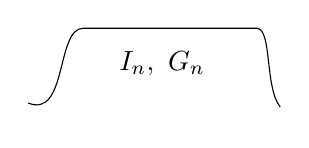
\begin{tikzpicture}[x=1cm,y=1cm]
\node at (1.7,0) {$I_n,\ G_n$};
\draw (0,-.5) .. controls (.5,-.7) and (.35,.45) .. (.7,.45) -- (2.9,.45) .. controls (3.1,.45) and (3,-.3) .. (3.2,-.55);
\end{tikzpicture}}

\uline{Prop 3.\unsure{2|1}.} Soit $f:X\to Y$ un morphisme fini, \unsure{($n$ un entier)}.

Conditions équivalentes

(i) $f$ est étale, et le rang de $X$ en un pt de $Y$ est partout égal à $n$.

(ii) Il existe un $Y_1-Y$ fid plat tel que $X\times_Y Y_1$ soit $Y_1$-isomorphe à $Y_1\times I_n$.

(ii bis) Kif-kif, avec $Y_1$ \deleted{\unsure{étale}} rev. étale galoisien (de groupe $G_n$ si on veut)

(iii) $X$ est isomorphe à un $P/\deleted{\unsure{G}}H$, où $P$ est un rev. étale galoisien de $Y$, de groupe $G$, et $H$ un sous-groupe de $G$.

(iii bis) Kif kif, avec $G=G_n$, $H=G_{\unsure{n-1,a|n-1}}$ \inserted{(une \unsure{dimension|diminution})} (stabilisateur d'un pt de $I_n$).

\figure{\begin{tikzpicture}[x=1cm,y=1cm]
\draw (0,4.8) -- (.18,.3) .. controls (.2,0) and (.35,.05) .. (.5,-.1);
\draw (-.7,5.8) .. controls (-.5,4.8) and (-1,3.6) .. (-.95,2.8) .. controls (-1.2,2) and (-.6,2.2) .. (-.7,1.5) .. controls (-.9,.4) and (-.4,-.6) .. (-.3,-1);
\end{tikzpicture}}

\margin{$\unsure{(i)|(iii)}\Rightarrow\unsure{(iii\ \mathrm{bis})|(ii\ \mathrm{bis})}$ \unsure{théorème de Galois},
$\unsure{(iii)}\Rightarrow(ii\ \mathrm{bis})$ immédiat
car les \uline{propriétés} des \uline{\unsure{morphismes}} sont \uline{compatibles} avec \uline{images réciproques}.
$(ii)\Rightarrow(i)$ par la descente.}

\[
(i)\Longrightarrow(iii\ \mathrm{bis})
\]
(la démonstration \inserted{ainsi que le résultat} qui suit, due à \inserted{J.P.} Serre).
On fait opérer $G_n$ sur $X\times\cdots\times X$ ($n$ facteurs, produit sur $Y$), de façon évidente.
L'ensemble des pts \unsure{d'inertie|d'isotropie} est \deleted{fermé et ouvert}\inserted{réunion de composantes} connexes (car si $s\in G_n$ est dans le groupe \unsure{d'inertie|d'isotropie} d'un pt $x$, il opère trivialement sur
\scanpage{154}
% archive foliation: 153
toute la composante connexe dudit point).
Soit $P$ son complémentaire. Il est \inserted{un rev. étale de $Y$,} stable sous $G_n$, qui y opère sans inertie.
De plus, en tout pt $y\in Y$, la \deleted{\unsure{fibre de}}\inserted{fibre} $P$ en $y$ a exactement $n!$ points géométriques --- car \deleted{\unsure{les}} \unsure{celui|ceux} $E$ de $\unsure{X^n|X}$ est isomorphe à $I_n$, donc \unsure{celui|ceux} de $X^n$ est \deleted{isomorphe}\inserted{\unsure{isomorphe|bijection}} comme ens. à opérateurs à $E^n\ \deleted{I_n^n}$, et on est à \unsure{enlever} les pts qui sont fixes sous des permutations non triviales de $I_n$: il reste les suites d'élém \uline{tous distincts} de $E$, il y en a $n!$.
En vertu de prop 2.5., $P$ est \deleted{donc}\inserted{un} revêtement étale galoisien de $Y$ de groupe $G_n$.

D'autre part, \deleted{\unsure{on sait}} la \deleted{première}\inserted{dernière} projection
$\operatorname{pr}_n:X^n\to X$ \deleted{\unsure{induit}} est invariante sous le stabilisateur $H=G_{n-1}$ de $\{n\}$, \deleted{\unsure{d'où un homom.}} il en est à fortiori de l'application induite sur $P$: $P\to X$, d'où un \deleted{\unsure{morphisme}} $Y$-\deleted{\unsure{hom.}}morphisme canonique
\[
\varphi:P/H\longrightarrow X.
\]
Comme $P/H$ est étale sur $\deleted{\unsure{Y|X}}$ (\uline{vérif}) \inserted{ainsi que $X$ \unsure{qui est un|d'où un} \unsure{morphisme} étale} pour montrer que $\varphi$ est un iso, il suffit de prouver
\margin{?\quad\unsure{?}}
\figure{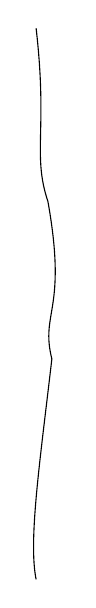
\begin{tikzpicture}[x=1cm,y=1cm]
\draw (0,7) .. controls (.15,5.7) and (-.05,5.4) .. (.15,4.8) .. controls (.4,3.4) and (.05,3.4) .. (.2,2.8) .. controls (.05,1.5) and (-.1,.5) .. (0,0);
\end{tikzpicture}}
\scanpage{155}
% archive foliation: 154
ramener au cas où $G$ opère transitivement sur l'ens des comp. connexes.
Soit $X_0$ \inserted{$(0\in I)$} une d'elles, $G_0$ son stabilisateur, alors il est évident que $X$ s'identifie à $\unsure{X|X_0}\times_{G_0}G$, et $X/G$ à $X_0/G_0$.
\deleted{Enfin, \unsure{donc}} on est ramené à $X_0$ connexe.
\deleted{Soit $H$ \unsure{$x\in X_0$}, soit $G_i$ son groupe d'inertie, il opère trivialt sur $X$ \unsure{puisque est connexe}.}
\deleted{\unsure{l'ens}}
On peut supposer que $G_0$ opère \uline{\unsure{fidelt}}.
Mais \uline{alors il opère sans inertie} donc $X\longrightarrow X/G$ est \uline{étale} (prop ---).

Reste à voir que $X/G$ est étale sur $Y$.

\margin{$*\quad\unsure{\prime}$}
\diagram{\begin{tikzcd}
X \arrow[dr] & \\
& X'=X/G \arrow[d] \\
& Y\ni y
\end{tikzcd}
\qquad
\begin{tikzcd}
k(x') \arrow[d,no head] \\
k(x) \arrow[d,no head] \\
k(y)
\end{tikzcd}}

Faisons une extension fid plate de la base $Y$ convenable, on est ramené au cas où l'ext résiduelle $k(x)/k(y)$ est triviale.
\unsure{Comme}, on voit sur le diagramme $\widehat{\mathcal O}_y\simeq\widehat{\mathcal O}_{x'}$, cqfd.

\diagram{\begin{tikzcd}[column sep=large]
\widehat{\mathcal O}_y \arrow[r,no head] \arrow[rr,bend right=25,"\sim"'] &
\widehat{\mathcal O}_{x'} \arrow[r,"\sim"] &
\widehat{\mathcal O}_x
\end{tikzcd}}

\uline{Corollaire}
\deleted{Soit} $X$ étale sur $Y$ en $x$, $q:X\to X'$ un $Y$-morphisme étale en $x$; alors $X'$ est étale sur $Y$ en $q(x)$.

\figure{\begin{tikzpicture}[x=1cm,y=1cm]
\draw (2.8,5.2) .. controls (1.9,4.8) and (2.6,3.8) .. (2.8,3) .. controls (3,2.1) and (3,1.2) .. (2,1) -- (1.4,1.2) .. controls (.1,.9) and (-.2,.2) .. (.4,0) .. controls (1.4,-.3) and (2.2,.1) .. (2.1,.9);
\end{tikzpicture}}
\scanpage{156}
% archive foliation: 155
qu'il est \uline{surjectif} et \uline{radiciel}, donc que pour tout $y\in Y$, la fibre géométrique de $P/H$ \deleted{\unsure{dans}} en $y$ s'envoie bijectivement sur celle de $X$ en $y$.
Or c'est encore un pt trivial, d'après l'explication précédente.

\margin{pts géométriques \unsure{en $y$} de $P/H$ $=$ \deleted{\unsure{pts géom.}} \unsure{les classes} \unsure{sous $H$} des pts géom. de $P$.}

Évident $(iii\ \mathrm{bis})\Rightarrow(iii)$, et $(iii)\Rightarrow(i)$ d'après un \uline{lemme} précédent, déjà utilisé.
D'où l'équivalence de $(i)\ (iii\ \mathrm{bis})\ (iii)$.

De plus $(iii)\deleted{\unsure{\Leftarrow}}\Rightarrow(ii\ \mathrm{bis})$, comme on voit en prenant $Y_1=P$, et utilisant la formule
$(X\times G)/H\simeq X\times G/H$, et $(ii\ \mathrm{bis})\Rightarrow(ii)$.
Enfin, $(ii\deleted{\mathrm{bis}})\Rightarrow(i)$ est immédiat
\deleted{[car la condition \unsure{loc.}}
Car si $X$ est défini par un faisceau d'alg $\underline A$ sur $Y$, $X_1$ le sera par son image réciproque $\underline A_1$.
Si $\underline A_1$ est loc. libre, il en est de $=$ de $\underline A$ comme bien connu.
Si les fibres de $X_1$ sur $Y_1$ sont séparables, \inserted{(déduites de celles de $X$ sur $Y$ par ext. des corps de base)} il en est de $=$ de celles de $X$ sur $Y$.
\uline{Donc} si $X_1$ est étale sur $Y_1$, $X$ l'est sur $Y$.
\margin{\uline{loc.}}

\uline{Cor}
Si $X$ est connexe, alors dans $(iii)$ on peut prendre $P$ \uline{connexe}.
\figure{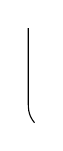
\begin{tikzpicture}[x=1cm,y=1cm]
\draw (0,.65) -- (0,-.3) .. controls (0,-.45) and (.04,-.5) .. (.08,-.55);
\end{tikzpicture}}
\scanpage{157}
% archive foliation: 156
\uline{Proposition 3.1.} (\unsure{Remonter}) $X$ étale sur $Y$ (\unsure{par ex. fini}).
$G$ groupe fini \deleted{de}\inserted{opérant par} $Y$-automorphismes de $X$.

\inserted{(i)} \deleted{Si $s\in$} L'ens des pts de $X$ où $G$ opère \inserted{\unsure{sans}} ramification est à la fois ouvert et fermé.
\margin{\unsure{sans inertie}}

(ii) \deleted{$\unsure{X/G\to X}$} $X/G$ existe, et $X\to X/G$ et $X/G-Y$ sont \uline{étales}.

\figure{\begin{tikzpicture}[x=1cm,y=1cm]
\draw (0,2) -- (0,1);
\draw[->] (.15,.7) .. controls (-.6,.1) and (-.25,.3) .. (.8,1);
\draw (0,0) -- (0,-.6);
\end{tikzpicture}}

Si $s\in G$ \deleted{\unsure{opère trivialt}} est dans le groupe d'inertie d'un pt $x\in X$, il \deleted{laisse fixe}\inserted{opère triv. sur tte} la composante connexe de $x$ (vérif), donc l'ens $X(s)$ des $x\in X$ tels que $s\in G_i(x)$ est une réunion de composantes connexes, donc ouvert et fermé.
Comme \deleted{$\unsure{X}$} l'ens des pts à $G_i(x)\ne e$ est la réunion des $X(s)$ $(s\ne e)$, (i) s'ensuit.
D'autre part, $X$ étant qu. affine sur $Y$, $X/G$ existe [---]
\deleted{donc} \unsure{on a} \unsure{finissons-en pour $(ii)$}.

Soit $I$ l'ens des comp. connexes de $X$.
$G$ opère sur $I$, \deleted{\unsure{et on est ramené à}}\inserted{et $X$ est réunion des}
\unsure{un|ens.} $\deleted{\unsure{X(\alpha)}}$ $\alpha\in I/G$, détermine un ouvert $X(\alpha)=\bigcup_{i\in\alpha}X_i$, stable sous $G$.
Donc $X/G=\bigcup X(\alpha)/G$ on est
\scanpage{158}
% archive foliation: 157
\uline{Catégorie galoisienne}

(i) Une catégorie $\mathcal C$

(ii) Un foncteur $F:\mathcal C\to\text{Ensembles finis}$

Axiomes:

\margin{\unsure{Poser} plutôt en axiome l'\uline{existence} d'un $F$ ayant les propriétés: \deleted{\unsure{Soit}} $F$ permute aux sommes, aux produits, aux \unsure{quotients par} groupes finis, et est tel qu'une \unsure{injection} $F(X)\to F(Y)$ \unsure{($X,Y$ conn.)|($X$ connex.)} $\Rightarrow X\overset{\sim}{\longrightarrow}Y$.}

(Gal 1) Dans $\mathcal C$, les sommes et les produits \deleted{de deux objets}\inserted{finis} existent [d'où l'existence de $\underline0$ et $\underline1$]

\deleted{(Gal 3) $X\in\mathcal C$, $F(X)=\varnothing\Longrightarrow X$ est une unité à gauche (soit $\underline0$)}

(Gal 4) $F$ permute à la somme et au produit

$X\in\mathcal C$ est dit \deleted{\uline{irréductible}}\inserted{connexe} si $X=X'\amalg X''$ implique $X'\simeq\underline0$ ou $X''\simeq\underline0$

(Gal 2) $X\in\mathcal C$ \deleted{$X\ne\underline0$} implique
\[
X\simeq\coprod_{i\in I}X_i,\quad \inserted{X_i\ne\underline0},
\]
et tte décomposition $X\simeq X'\amalg X''$ s'explique
\[
X'\simeq\coprod_{i\in I'}X_i,\quad X''=\coprod_{i\in I''}X_i,\quad
I'\cap I''=\varnothing,\quad I'\cup I''=I.
\]
Les $X_i$, déterminés de façon essentiellement unique [avec les $X_i\to X$] sont appelés les \uline{comp.} \deleted{\uline{irréductibles}}\inserted{connexes} de $X'$ [N.B. $X=\underline0\Longleftrightarrow I=\varnothing$]

(\uuline{Gal 3}) Soit $f:X\to Y$ avec $Y$ \deleted{irréductible}\inserted{connexe $\ne\underline0$}.
Alors les composantes \inserted{connexes} $X_i$ de $X$ telles que $f$ induise un \uline{isom.} $f_i:X_i\overset{\sim}{\longrightarrow}Y$ sont en correspondance biunivoque avec les \uline{sections} $g_i:Y\to X$ \deleted{$\unsure{f}$}
[hom. tels que $fg=\operatorname{id}_Y$], $g_i$ étant le composé \deleted{\unsure{de}}
\diagram{\begin{tikzcd}
Y \arrow[r,"f_i^{-1}"] & X_i \arrow[r,"\text{inj. can.}"] & X
\end{tikzcd}}
[en d'autres termes, toute section se factorise]
[N.B. il suffit de le vérifier si $X=Z\times Y$, $f=p_2$]

\margin{Gal 3 et Gal 5 ensemble sont impliqués par:
Si $f:X\to Y$ est tel que $F(X)\to F(Y)$ soit \uline{injectif} (\deleted{\unsure{$Y$ connexe}}\inserted{$X,\deleted{\unsure{Y}}$ \unsure{connexe|connexes}}) alors c'est un isomorphisme \inserted{de} $X$ sur une composante connexe $Y_i$.}

(Gal 5) Dans les conditions de Gal 3, si \deleted{\unsure{le morphisme}}\inserted{$X,Y$ connexes et} $f:X\to Y$ induit $F(X)\overset{\sim}{\longrightarrow}F(Y)$, c'est un isomorphisme
[implique $F(X)=\varnothing\longrightarrow X=\underline0$]
[Il suffit de vérifier Gal 5 quand $X$ est une composante connexe d'un produit $Z\times Y$, $f$ étant induit par $p_2$]

(\uuline{Gal 6}) Soit $X\in\mathcal C$, $X$ connexe $\ne\underline0$, et \uline{galoisien}, \deleted{\unsure{c.à.d.}} i.e. \deleted{\unsure{Alors}} $G=\operatorname{Aut}(X)$ opère \uline{transitivement} dans $F(X)$.
\deleted{Tte composante \unsure{connexe d'un revêtement est galoisienne}}
Alors pour tout sous-groupe $H$ de $G$, $X/H$ dans $\mathcal C$ \uline{existe}, et
\[
\unsure{E(X/H)|F(X/H)}\simeq F(X)/H.
\]
\scanpage{159}
% archive foliation: 158
Catégorie $\mathcal C$, sous-catégorie $\mathcal P_{\unsure{1}}$ (pleine), morphismes ``non ramifiés''

\uline{$1^\circ$} Dans $\mathcal C$, les sommes finies existent, ainsi que les produits fibrés.

\uline{$4^\circ$} Dans $\mathcal C$, le \deleted{produit}\inserted{composé} de deux morphismes non ramifiés \inserted{les morphismes identiques}, ou l'image inverse d'un morphisme non ramifié, sont non ramifiés.

\uline{$5^\circ$} \deleted{\unsure{les}} $f:X\to Y$ est non ramifié $\Longleftrightarrow$ les $f|X_i$ ($X_i$ les comp. connexes) \deleted{\unsure{les sommes $\coprod(f_i:X_i\to Y)$}} non ramifiés.

\uline{$2^\circ$} Dans $\mathcal C$, il y a des composantes connexes.

\uline{$3^\circ$} Les \deleted{pts} $\xi\in\mathcal P$ sont connexes
(donc $\operatorname{Hom}(\xi,X\amalg Y)=\operatorname{Hom}(\xi,X)\amalg\operatorname{Hom}(\xi,Y)$]

\uline{$6^\circ$} Pour tout $f:X\to Y$ non ramifié, \inserted{$Y$ connexe}, et $\xi\in\mathcal P$,
$\operatorname{Hom}(\xi,X)\to\operatorname{Hom}(\xi,Y)$ est \uline{surjectif}.

\uline{$7^\circ$} Si \deleted{$X$} et $Y$ sont connexes, et la fibre de
$\operatorname{Hom}(\xi,X)\to\operatorname{Hom}(\xi,Y)$ est réduite à un élément, alors $f$ est un \uline{isom}
(on suppose $f$ non ramifié, $\xi\in\mathcal P$)

\uline{$8^\circ$} Si $f:X\to Y$ non ramifié, $Y$ connexe, alors \deleted{pour} toute \deleted{\unsure{les}} section $s:Y\to X$ est un \uline{isom.} de $Y$ sur une composante connexe de $X$.

\uline{$9^\circ$} Soit \deleted{$G$ \inserted{groupe fini} opère dans $X$ ``sans \unsure{points}''}
$f:X\to Y$ \uline{non ramifié}, et $X$ connexe, \unsure{$\xi\in$} $e\in\operatorname{Hom}(\xi,Y)=Y^\xi$, tel que $G=\operatorname{Aut}_Y(X)$ opère transitivement dans $(f^\xi)^{-1}(e)$.
Alors pour tout sous-groupe $H$ de $G$, $X/H$ existe \inserted{dans $\mathcal C$}, et est un revêtement non ramifié de $Y$.
\deleted{et $X\to\unsure{X/H}$ \unsure{est non ramifié}}
et deux élts de $\operatorname{Hom}_{\unsure{Y}}(\xi,X)$ au-dessus de $e$ ayant $=$ image par $X\to X/H$ sont congrus mod $H$.

Sous ces conditions, pour $x\in\operatorname{Hom}(\xi,X)$ on définit $\pi_1(X,x)$.
Il ne change pas si on remplace $\xi$ par $\xi'$ tel que $\xi'-\xi$ soit donné.
C'est un foncteur \uline{covariant} en $(X,x)$

\diagram{\begin{tikzcd}
\xi \arrow[r,"x"] \arrow[d] & X \arrow[d] \\
\xi' \arrow[r,no head,"x'"] & X'
\end{tikzcd}}
définissant $\pi_1(X,x)\mathbin{\unsure{-|\to}}\pi_1(X',x')$.

\uline{Etc.}
\scanpage{160}
% archive foliation: 159
Groupe fondamental dans les catégories.

$\mathcal C$ une catégorie, avec une famille $(D)$ de morphismes dans $\mathcal C$, satisfaisant aux conditions usuelles

(i) Contient identité et stable par composition

(ii) Stable par changement de base

On suppose de plus

(iii) \inserted{$(D)$} \unsure{Ce} sont des morphismes de descente [donc des épimorphismes stricts \inserted{universels} si \inserted{\uline{on suppose que}} \uline{les produits et produits fibrés existent}].
Enfin, on suppose

\figure{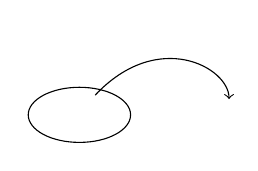
\begin{tikzpicture}[x=1cm,y=1cm]
\draw (0,0) ellipse (.65 and .35);
\draw[->] (.2,.25) .. controls (1,1.1) and (1.9,.6) .. (1.9,.2);
\end{tikzpicture}}

\margin{On peut avoir $\mathcal C$ \unsure{restreint}, en introduisant de \unsure{façon} \deleted{\unsure{connue}} une classe de morphismes $(D)$ [des morphismes \unsure{permettant} \unsure{(i), (ii)}].}

(iv) On peut ``descendre'' un $g\in(D)$ par un $f\in(D)$
[mais on ne suppose pas qu'on peut descendre \uline{tout} morphisme par un $f\in(D)$].

\uline{Dans la suite, $D$ est supposé donné une fois pour toutes.}

\uline{On suppose que dans $\mathcal C$ les sommes finies} [resp. quelconques] existent
\inserted{et \unsure{satisfont à certaines conditions}}.

\margin{\fbox{\parbox{.3\linewidth}{(v) La projection $X\times I\longrightarrow X$ est $\in(D)$.}}}

\uline{Exemple}
Catégor. $\mathcal C$ des préschémas. \deleted{La catégorie}
Classe $(D)$ des morphismes \uline{plats} et \uline{affines}.
[ou \uline{plats} et quasi-projectifs].

On va développer une théorie particulière de fibrés principaux [vérifiant les conditions générales \deleted{\unsure{correspondantes}} d'une théorie de fibrés principaux, cf. ---].

\uline{Groupes structuraux}: $X\times G$\qquad $G$ un groupe ordinaire fini [\unsure{resp.!} quelconque]

\uline{Fibrés principaux \unsure{bons} sur $X$}, de groupe $G$: les fibrés \uline{formels} ainsi, avec hom $P\to X$ $\in(D)$
\scanpage{161}
% archive foliation: 160
\uline{Espaces à opérateurs admissibles}: Le morphisme $E\to X$ est $\in D$.

\uline{Hom admissibles} de \deleted{groupes} \uline{faisceaux structuraux}: se déduit \uline{d'un hom de groupes usuels}.

\deleted{Hom} \uline{Inclusions admissibles}: les monomorphismes de groupes ordinaires.
% Faint reversed show-through from the opposite side is not a second inscription.
\scanpage{162}
% archive foliation: 161
Soit $f:X-Y$ un morphisme \inserted{propre} dominant, $Y$ \inserted{loc. noeth.} \uline{normal} \uline{connexe}.
Alors $\pi_1(X)\to\pi_1(Y)$ a un conoyau fini
(regardons le pt générique $\eta$ de $Y$, et sachant que $\pi_1(\eta)\to\pi_1(Y)$ est surjectif, on est ramené au cas où $Y=\operatorname{Spec}(K)$.
On voit de $=$ qu'on peut supposer $X$ séparable sur $\unsure{k|K}$ et abs\textsuperscript{t} connexe
[remplacer $K$ par une extension \inserted{séparable} finie convenable $K'$], et diviser $\mathcal O_{X'}$ par ses élts nilpotents, \unsure{enfin} prendre une composante connexe de $X'$].
Mais alors $\pi_1(X)\longrightarrow\pi_1(Y)$ est \uline{surjectif}.

\figure{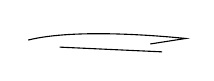
\begin{tikzpicture}[x=1cm,y=1cm]
\draw (0,0) .. controls (.6,.15) and (1.7,.05) .. (2,.02) -- (1.55,-.05);
\draw (.4,-.09) -- (1.7,-.15);
\end{tikzpicture}}

N.B. Si $Y$ n'est pas \uline{normal}, le th. est faux, $=$ si p.ex $X$ est la normalisée de $Y$.
Ex. $Y$ courbe int. sur $k$ alg. clos, avec pt double ordinaire, $X'$ sa normalisée.
On a $\pi_1(\unsure{Y'|X'})=0$, $\pi_1(Y)=\widehat{\mathbb Z}$
\unsure{prouvé} \unsure{en} \deleted{\unsure{se}} par \unsure{comparaison}.

\figure{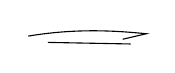
\begin{tikzpicture}[x=1cm,y=1cm]
\draw (0,0) .. controls (.6,.1) and (1.1,.07) .. (1.5,.03) -- (1.2,-.04);
\draw (.25,-.08) -- (1.3,-.1);
\end{tikzpicture}}

On voit facilement que dans le dernier exemple, on ne peut former $\underline{\operatorname{Hom}}_Y(X,Y\amalg Y)$
[car en un \inserted{certain} pt $y_0$ de $Y$, il y a deux pts géométriques dans l'image inverse, alors qu'il n'y en a qu'un au voisinage].
\uline{Supposons cependant} $f:X\to Y$ \uline{universellement ouvert} [p. ex. $Y$ normale], je crois que
\scanpage{163}
% archive foliation: 162
peut alors \deleted{\unsure{dans $f$}} construire les $f_*(X_1)$ pour $X_1$ étale sur $X$.
\unsure{Par les plats)}

\diagram{\fbox{$\begin{tikzcd}[column sep=large,row sep=small]
& X \arrow[d] \\
S & Y \arrow[l,very thick]
\end{tikzcd}$}}
% Faint reversed writing below is show-through from the opposite side.
\scanpage{164}
% archive foliation: 163
\deleted{\unsure{pro Groupe}}

\uline{Progroupe fondamental}

\uline{pour les revêtements}

\uline{infinis} \uline{principaux}
\scanpage{165}
% archive foliation: 164
Le $\widetilde{\pi}_1(S,\xi)$, $S$ préschéma. connexe, $\xi$ pt géom.

Pour tout groupe $\pi$, soit
\[
\Pi^1(S,\xi;\pi)
\]
l'ens des classes, à isom près, de \deleted{rev.}\inserted{fibrés} principaux homogènes sur $S$, de groupe structural $\pi$, pointés au dessus de $\xi$.

(i) $\pi\mapsto\Pi^1(S,\xi;\pi)$ est exact à gauche.

En effet a) Commute aux produits finis c'est trivial

b) Transforme un mono \inserted{$\pi\mathbin{-}\pi'$} en mono.

En effet, cela provient que pour \deleted{\unsure{un}} \inserted{\unsure{si}} \deleted{isom}
$P_1'\overset{u'}{\longrightarrow}P_2'$ de \inserted{deux} $\pi'$ fibrés \unsure{isom.}, il existe un et un seul \unsure{tel} isom qui applique $\xi_1'$ en $\xi_2'$.
Si alors $P_1'$ et $P_2'$ sont \uline{associés} à $P_1$, $P_2$ d'où
\[
\left\{\begin{array}{l}
P_i\subset P_i'\\
\xi_i=\xi_i'
\end{array}\right.,
\]
\deleted{donc} je dis que $u$ \deleted{applique} \deleted{\unsure{$f_i$}} induit un isom $u:P_1\mathbin{\unsure{-|\to}}P_2$.
En effet, \deleted{$P_i$ est ouvert et fermé dans $P_i'$, et contient $\xi_i$}
$\inserted{u'^{-1}(P_2)}$ est \uline{ouvert} et \uline{fermé} dans $P_1'$, et contient $\xi_1$, \unsure{alors il s'ensuit}
\scanpage{166}
% archive foliation: 165
\deleted{$\unsure{\Pi}$.\ \unsure{Je|S}} $P_i$ se déduit de $P_i'$ par une \uline{section} de $P_i'/\pi$ passant par $\unsure{\bar\xi'|\bar\xi_i'}$. $S$ étant connexe, il ne peut y en avoir qu'une seule telle section.

c) Si $\pi\mathbin{-}\pi'\rightrightarrows\pi''$ est exacte, alors \deleted{$\unsure{\Pi|\Phi}$} $\Phi(\pi)\mathbin{-}\Phi(\pi')\rightrightarrows\Phi(\pi'')$ aussi.

Il \deleted{\unsure{reste}} à prouver que si $P'$ de groupe $\pi'$, pt marqué $\xi'$, est tel que \deleted{\unsure{on}} l'on ait un isom
\[
P'\times_{\pi'}(\pi'',\varphi_1)\xrightarrow[\sim]{u}
P'\times_{\pi'}(\pi'',\varphi_2),
\]
alors on peut restreindre le groupe structural.

Or soit $Q$ le sous-schéma de $P'$ des coïncidences de $u i_1$ et $i_2$. Il est ouvert et fermé, contient $\xi'$, est stable par $\pi$, donc correspond à un sous-schéma de $P'/\pi$ à la fois ouvert et fermé $S'$ [donc \inserted{absolument} fidèlement plat et quasi-compact].

\margin{\diagram{\begin{tikzcd}
\pi \arrow[r,dash] & \pi' \arrow[r,shift left=.5ex] \arrow[r,shift right=.5ex] & \pi''
\end{tikzcd}}
\diagram{\begin{tikzcd}
P' \arrow[r,"i_1"] \arrow[dr,"i_2"'] & P_1'' \arrow[d,"u"]\\
& P_2''
\end{tikzcd}}}

De plus, on voit que les \deleted{\unsure{deux}} fibres géom de $S'\mathbin{-}S$ ont \unsure{partout} un pt; donc c'est un isom $S'\to S$ \unsure{alors}, \unsure{on gagne}\ldots
\scanpage{167}
% archive foliation: 166
\inserted{Supposons \deleted{$\unsure{S}$} $S$ loc. noeth \uline{ou} $\pi$ artinien [condition des chaînes descendantes].}

(ii) Tout élément $c\in\Phi(\pi)$ est induit par un élément \unsure{minimal}, $c'\in\Phi(\pi')$.

\margin{\unsure{pour que} $\unsure{\Phi(\pi)}$ \unsure{ait un} \uline{\unsure{élémt}}}

En effet, si $c$ correspond à $P,\xi$, supposons \inserted{\unsure{corresp. d'élémts|corresp. d'éléments}} qu'il puisse \deleted{\unsure{être}} \unsure{réduire} à $P',\xi'$ \inserted{[groupe $\pi'\subset\pi$]} et $(P'',\xi'')$ [groupe $\pi''\subset\pi$].
Considérons
\[
P/_{\pi'\cap\pi''}\longrightarrow P/_{\pi'}\times P/_{\pi''}
\]
\margin{$\pi/_{\pi'\cap\pi''}\to\pi/_{\pi'}\times\pi/_{\pi''}$}
c'est une imm. ouverte et fermée, et d'autre part on a une section du $2^\circ$ \unsure{mbr|mb.} qui \deleted{est} au pt $(\xi',\xi'')$ est dans l'image du premier, elle y est donc partout.

Donc on peut restreindre le groupe structural à $\pi'\cap\pi''$. Donc les groupes auxquels on peut restreindre forment un ens filtrant décroissant, $\pi_i,\ldots$, donc $P_i\subset P$ forment un syst. projectif.

Si \deleted{\unsure{les groupes}} $\pi$ est artinien, \unsure{on gagne}. Le système des $P_i$ est \deleted{\unsure{les uns inclus dans les autres} $P_i$ \unsure{est}} stationnaire. Si $S$ est loc. noeth., \deleted{\unsure{on}} \deleted{fini. Donc on peut former le préschéma $\varprojlim_i P_i$ qui est \unsure{encore fibré sur} $P$, \deleted{\unsure{le groupe est}} \inserted{et qui comme sous-pré\-schéma est} ouvert et fermé, et est un fibré}
\scanpage{168}
% archive foliation: 167
\deleted{principal homogène sous $\pi'=\bigcap\pi_i$. On \unsure{sait} ici que la question est locale sur $S$ [\unsure{la pro. de la descente finie}] donc on peut supposer $S$ \uline{affine}. Mais alors il existe $S^{(0)}$ de type fini sur $\mathbf Z$, \inserted{connexe}, et $(P^{(0)},\xi^{(0)})$ principal homogène \deleted{\unsure{constant}} sous $\unsure{\pi_{S^{(0)}}}$, qui donne $P$ par extension de la base [se rappeler que $P$ est trivialisé par $S'\mathbin{-}S$ qu. fini étale !]. On peut supposer $S^0$ \uline{connexe}.

\diagram{\begin{tikzcd}
P^\circ \arrow[d] & P \arrow[l] \arrow[d]\\
S^\circ & S \arrow[l]
\end{tikzcd}}
Alors les}

\unsure{l'on fait maintenant comme suit}: on regarde la composante connexe $P^\circ$ de $\xi$ dans $P$ [\deleted{\unsure{elle est}} est \uline{ouverte et fermée}, car $P$ est loc. noeth donc loc. connexe]. Je dis que $P^\circ\to S$ est \uline{surjectif}. Comme l'image est ouverte, pour prouver qu'elle est fermée, on est ramené au cas d'un anneau de valuation discret complet \inserted{à corps résiduel alg clos}: à prouver que si $P$ est un fibré principal homo sur $S$
\scanpage{169}
% archive foliation: 168
\uline{Application} Un revêt. étale \inserted{\uline{$T$ sur $S$}} est dit à \uline{groupe structural} $\pi$, \inserted{\fbox{fibre $F$}}, \deleted{\unsure{si on a fixé un} sous-schéma de $\operatorname{Aut}_S(T)$, qui est} \unsure{si on a} donné une opération fidèle de $\pi$ sur $F$, et un sous-fibré \inserted{$\pi_S$} principal de $\underline{\operatorname{Isom}}_S(E_S,T)$. Si $S$ est connexe et muni d'un pt géométrique $\xi$, il revient au $=$ de se donner un $T$ avec une telle structure, ou de se donner des opérations \deleted{continues} de $\widetilde\pi_1(S,\xi)$ \deleted{\unsure{à travers}} sur $F$ :
\[
\text{hom}\qquad\widetilde\pi_1(S,\xi)\longrightarrow\deleted{\unsure{G}}\pi.
\]

\uline{\unsure{Exemple|Exemples}} Schémas en groupes comm., constants tordus sur $S$, \deleted{à fibre \unsure{de}} \unsure{génération} finie sur $S$, correspondent \deleted{aux} $(\widetilde\pi_1(S,\xi))$-Modules admissibles \deleted{de \unsure{présent}} qui sont des $\mathbf Z$-modules de type fini.
\scanpage{170}
% archive foliation: 169
de groupe un groupe constant $\uline{\pi_S}$, alors \unsure{tte} \uline{composante connexe} $P^\circ$ se surjecte sur $S$. Or c'est bien, car $P$ est \uline{trivial} !

Ceci étant, comme $P^{(0)}\subset\bigcap P^{(i)}$ pour \unsure{tt} $i$, on voit que $\bigcap_i P^{(i)}$ contient un pt de chaque fibre. \deleted{\unsure{En effet l'intersection}} \deleted{Il s'ensuit que} \deleted{\unsure{puisque}} \deleted{\unsure{les}} \inserted{chaque} $P^{(i)}$ est une réunion de composantes connexes de $P$, il en est de $=$ de l'intersection, \deleted{qui} $P'$, qui contient $\xi^\circ$. Elle est stable par $\pi'$, et on constate aussitôt (en regardant sur chaque fibre géométrique, et utilisant que $P'_{\bar s}\ne\varnothing$) que $P'$ est fibré principal homogène sous $\pi'$.
cqfd.

\uline{Conséquences} Si $\pi$ varie dans \inserted{une sous-}catégorie des groupes artiniens, \deleted{\unsure{et si}} stable par produits finis et sous-groupes, ou si $\pi$ varie ds n'importe quelle catégorie stable par ces opérations, mais $S$ étant loc. noeth --- alors le foncteur $\pi\mapsto\Pi^1(S,\xi;\pi)$ est strictement pro-représentable.

\margin{\unsure{On aura} pro-groupe $\widetilde\pi_1(S,\xi)$ [qui ne peut plus être interprété comme un simple groupe topologique].}
\scanpage{171}
% archive foliation: 170
\uline{Groupe fondamental} : (\unsure{Revêtts} infinis)

$S$ préschéma. Pour tout groupe discret $G$, on définit
\[
H^1_C(S,G)=\varinjlim_{T/S\in C}H^1(T/S,G)
\]
\deleted{$T$ \unsure{fid plat de type f. sur $S$}}\quad
\deleted{\unsure{fid plat sur $S$}}

où
\[
H^1(T/S,G)=H^1(K_{T/S},G)=H^1(\pi_0(K_{T/S}),G)
\]
où $C$ est une catégorie de $S$-préschémas.
Les cas les plus importants sont les suivants
\diagram{\[
\begin{array}{l}
\left\{\begin{array}{lll}
\text{(i)}&C_1&\text{$S$-préschémas fid plats quasi-compacts, \deleted{\unsure{loc. noeth.}}}\\[3pt]
\multicolumn{3}{l}{\left.\begin{array}{lll}
\text{(ii)}&C_2&\rule{3cm}{.3pt}\quad\text{de type fini}\\[3pt]
\text{(iii)}&C_3&\rule{3cm}{.3pt}\quad\text{quasi-finis}
\end{array}\right\}}
\end{array}\right.\\[6pt]
\left.\begin{array}{lll}
\text{(iv)}&C_4&\rule{3cm}{.3pt}\quad\text{finis par morceaux}\\[3pt]
\text{(v)}&C_5&\rule{3cm}{.3pt}\ \deleted{\unsure{\text{étales}}}\quad\text{finis étales p. morceaux}
\end{array}\right\}
\end{array}
\]}

\margin{élucider ici les questions d'effectivité des données de descente\ldots\ \unsure{les ramener} à la descente des morphismes étales de type fini\ldots}

On a donc
\[
H^1_{C_i}(\deleted{\unsure{T}}S,G)\hookrightarrow H^1_{C_j}(S,G)\qquad\text{si }i\geq j
\]
application injective canonique. \uline{Si $G$ est fini}, alors tous les hom sont bijectifs, et $H^1(S,G)$ est l'ensemble des classes (à isom près) des revêtements étales galoisiens de groupe $G$, donc $\simeq\operatorname{Hom}(\pi_1(S,a),G)/\operatorname{int}(G)$. Notre intérêt ici est dans le cas $G$ infini. Notons en passant
\[
H^1_{C_3}\simeq H^1_{C_2}.
\]
\scanpage{172}
% archive foliation: 171
et si $S$ est le spectre d'un anneau de Dedekind
\[
H^1_{C_2}\xrightarrow{\sim}H^1_{C_1}
\]
[d'où dans ce cas $H^1_{C_3}\xrightarrow{\sim}H^1_{C_2}\simeq H^1_{C_1}$].
Si $S$ est le spectre d'un anneau \deleted{local complet} \inserted{de valuation} discrète à corps résiduel alg. clos $V$, on aura de $=$
\[
H^1_{C_i}\unsure{S|\delta}\simeq H^1_{\deleted{\unsure{C_i}}}(\widehat V/V,-)
\qquad\text{pour }i=1,2,3
\]

Si $S$ est le spectre d'un anneau local \uline{complet} $V_{\unsure{\varphi}}$, alors
\[
\deleted{\unsure{H^1_{C_4}(\widehat V/V,G)\simeq}}
\]
\[
H^1_{C_5}\simeq H^1_{C_4}\simeq H^1_{C_3}\quad(\simeq H^1_{C_2})
\]
et on aura de plus
\[
H^1_{C_i}(V,-)\simeq H^1_{C_i}
(\underset{\substack{\downarrow\\\text{corps}\\\text{résiduel}}}{k},-)
\qquad(i=2,3,4,5)
\]
\scanpage{173}
% archive foliation: 172
Plan
\scanpage{174}
% archive foliation: 173
\uline{Groupe fondamental}

I\quad \deleted{\uline{\unsure{Th de comparaison}} premier}
\inserted{Premier th. de changement de base pour $\pi_1$}
(ou th. de comparaison)

II\quad Deuxième th. de changement de base pour $\pi_1$

1) Morphismes $(-1)$-connexes et $0$-connexes

2) Morphismes locaux $(-1)$-connexes et $0$-connexes.

3) \deleted{Une} Caractérisation des morphismes locaux ou globaux $i$-connexes $(i=0,1)$.

4) Le deuxième théorème de \deleted{comparaison} \inserted{changement de base pour $\pi_1$ :} énoncés et corollaires\ldots

5) \deleted{Lemmes, et} Démonstration du théorème.

6) Généralisations à l'aide de la résolution des singularités.

7) Applications : la dimension cohomologique de certains corps\ldots
\scanpage{175}
% archive foliation: 174
$\unsure{\pi_2|\Pi_2}$
\scanpage{176}
% archive foliation: 175
\diagram{\begin{tikzcd}[column sep=small]
& \widetilde X^u \arrow[d] &&\\
\widetilde\pi\Biggl( & \widetilde X^h \arrow[d] &
\Biggr)\widehat{\widetilde\pi}=\pi & \widetilde X \arrow[d,dash]\\
& X^h \arrow[rr] && X
\end{tikzcd}}
\[
\Pi^{\unsure{I|2}}(X,G)\simeq H^{\unsure{2|1}}(\widetilde X,G)
\simeq\underset{\rule{1cm}{.3pt}}{\lim}H^2(X_i,G)
\simeq\varinjlim H^2(\widetilde X_i,G)
\]
\margin{$\widetilde\pi/H_i=\pi_i$}
\[
H^*(\widetilde X_{\unsure{j|i}},G)\Longleftarrow E^{pq}_2
=H^p(H_i,H^q(\widetilde X,G))
\]
\[
\unsure{H^*|\Pi^*}(\widetilde X_{\unsure{j|i}},G)
\Longleftarrow E^{pq}_2
=\underset{i}{\underline{\lim}} H^p(H_i,H^q(\widetilde X,G))
\]
\figure{\begin{tikzpicture}[x=.55cm,y=.55cm]
\draw (0,0)--(4.5,0);
\draw (0,0)--(0,4.1);
\node[above] at(-.2,4.1){$q$};
\node[right] at(4.6,-.1){$p$};
\foreach \x in {0,1,2,3}{\fill (\x,0) circle (.085);}
\foreach \x in {0,1,2}{\fill (\x,1.65) circle (.085);
\draw (\x-.09,.74)--(\x+.09,.92);
\draw (\x-.09,.92)--(\x+.09,.74);}
\node at(4.2,3.3){$\unsure{E^p|E_2}$};
\end{tikzpicture}}

\diagram{\begin{tikzpicture}
\node[inner sep=0pt] at(0,0) {\begin{tikzcd}[column sep=small]
\bullet \arrow[r,dash]&
|[draw,ellipse,inner sep=7pt]| \underline{\lim} H^2(H_i,G) \arrow[r]&
\Pi^2(X,G) \arrow[r]&
\begin{array}{c}
\underset{i}{\underline{\lim}} H^2(\widetilde X_{\unsure{i}}^h,G)^{H_i}\\
\Vert\\
\Pi^2(X^h,G)
\end{array}\arrow[r]&
|[draw,ellipse,inner sep=8pt]|
\begin{array}{c}
\underline{\lim} H^3(H_i,G)\\
\downarrow\\
H^3(\widetilde X,G)
\end{array}
\end{tikzcd}};
\draw (-10.5,.65)--(-10.5,-1.4)
.. controls (-10.5,-2) and (-10,-2) .. (-9.5,-2)
--(10,-2);
\node[below] at(2,-2){$\pi_2(X)\longrightarrow G$};
\end{tikzpicture}}
\[
H^*(X^h,G)\Longleftarrow H
\]
\[
\operatorname{Ker}\bigl(\Pi^2(X,G)\to\Pi^2(X^h,G)\bigr)
\simeq\underset{i}{\underline{\lim}} H^2(H_i,G)
\]
\[
\operatorname{Coker}(\qquad\text{id}\qquad)
\simeq\operatorname{Ker}\left[
\begin{array}{c}
\underline{\lim} H^3(H_i,G)\\
\longrightarrow H^3(\widetilde X,G)
\end{array}\right]
\]
\scanpage{177}
% archive foliation: 176
\diagram{\begin{tikzcd}
& Z' & Z_1''\unsure{\simeq|\cong} Z_2'' &\\
X \arrow[d] & X' \arrow[l] \arrow[d] &
X'' \arrow[l,shift left=.5ex] \arrow[l,shift right=.5ex] \arrow[d] &\\
Y & Y' \arrow[l] \arrow[d,equal] &
Y'' \arrow[l,shift left=.5ex] \arrow[l,shift right=.5ex] &\\
& X & \deleted{\unsure{\widetilde Y''|Y''}} & \widetilde Y'' \arrow[ul]
\end{tikzcd}}

\diagram{\begin{tikzcd}
\pi_1(\bar F)\arrow[r]\arrow[dr]&\pi_1(X)\arrow[r]\arrow[d,dotted]&\pi_1(Y)\arrow[r]&e\\
&G&&
\end{tikzcd}}
\[
\pi_1(Y)\longrightarrow G^{\pi_1(X)}
\]
\diagram{\begin{tikzcd}[column sep=small]
H^1(\pi_1(X),G)\arrow[r]&H^1(\pi_1(\bar F),G)^{\pi_1(Y)}\\
H^1(\pi_1(Y),G^{\pi_1(\bar F)})\arrow[u]&
{}=H^1(\pi_{\deleted{\unsure{1}}1}(Y),\unsure{\mathfrak z|\zeta})
\end{tikzcd}}
\[
\pi_1(Y)\longrightarrow\unsure{\mathfrak z|\zeta}
\]
\[
H^1(\pi_1(\bar F),G)
\]
\[
\pi_1(Y')\longrightarrow\unsure{\mathfrak z|\zeta}
\]
\[
H^1\left(Y'/Y,\operatorname{Hom}
\left(\overset{\deleted{\unsure{H^1}}}{\overbrace{\pi_1(\bar F)}},\unsure{\mathfrak z|\zeta}\right)\right)=0
\]
\diagram{\begin{tikzcd}
\pi_1(\unsure{Y|X})&
\pi_1(Y')\arrow[l]&
\pi_1(Y'')\arrow[l,shift left=.5ex]\arrow[l,shift right=.5ex]\arrow[dr]&
\pi_1(Y''')\arrow[l,shift left=1ex]\arrow[l]\arrow[l,shift right=1ex]\\
&&&\unsure{\mathfrak z|\zeta}
\end{tikzcd}}
\scanpage{178}
% archive foliation: 177
$\pi_0,\pi_1$ \uline{et formalisme}\\
\uline{simplicial}

(Revêtements infinis)
\scanpage{179}
% archive foliation: 178
\uline{Proposition} $S$ un préschéma \uline{connexe},
$S'$ un préschéma sur $S$ tel que $S'\to S$ soit \uline{submersif}
[p.ex. fid plat et quasi-compact, ou propre surjectif].
$S'',S'''$ les carré, cube fibré.

On suppose que $S'$ est \uline{somme} de \uline{préschémas connexes}
(i.e. ses composantes connexes sont ouvertes, i.e. $\pi_0(S')$ discret),
\deleted{et l'ens des \unsure{composantes connexes} de $S''$ est \unsure{q.c.}}

Soit $\xi$ un pt [géométrique] de $S$. Alors pour un groupe discret $G$ variable, le foncteur
\[
G\longmapsto\Pi^1(S'/S,\xi;G)
\]
\deleted{\unsure{considérons}} [où $\Pi^1(S'/S,\xi;G)$ désigne l'ens des classes, à isom près, des données de descente sur $G_{S'}$ \inserted{(fibré principal trivial)} relativement à $S'\to S$, pointées sur $\xi$] est strict$^{\mathrm t}$ proreprésentable :
\[
\Pi^1(S'/S,\xi;G)=\varinjlim\operatorname{Hom}(\pi_i,G)
\]

Si $\pi_0(S'')$ est \inserted{quasi-}\uline{compact}, i.e. tte fonction loc constante sur $\pi_0(S'')$ \unsure{n'a qu'un nb fini de valeurs}, --- p.ex. $S''$ quasi-compact]
\deleted{\unsure{ou $S''$ a}} \deleted{[un nb fini de comp. de connexité]}
\uline{alors} les $\pi_i$ sont de type fini. Si $S''$ a un nb fini \inserted{$n''$} de composantes connexes, alors le foncteur précédent est représentable : \deleted{de façon} \deleted{par}
\[
\Pi^1(S'/S,\xi;G)\simeq\operatorname{Hom}(\pi_1(S'/S,\xi),G)
\]
avec $\pi_1(S'/S,\xi)$ \deleted{\unsure{groupe}} \inserted{groupe discret} de type fini.
De façon précise, * Si \unsure{le nb} $n'$ des comp. conn. de $S'$ est aussi fini, et \deleted{$\unsure{n''-n'}$} $\pi_1(S'/S;\xi)$ est engendré par $\unsure{n''-n'}$ générateurs.
\scanpage{180}
% archive foliation: 179
\uline{Enfin}, considérons le sous-foncteur
\[
G\rightsquigarrow \Pi^1_{\mathrm{eff}}(S'/S,\xi;G)
\]
correspondant aux données de descente \uline{effectives}, pointées sur $\xi$.
\deleted{\unsure{Ce sont les $\Pi_0$}}
\unsure{(triviaux)}
Ce foncteur est également proreprésentable
[par un système projectif de quotients des $\pi_i$].

\uline{N.B.} J'ignore, $=$ si $S,S',S''$ noethériens, si ce dernier foncteur
est $=$ \uline{représentable}, à fortiori
(comme $\Pi^1(S'/S,\xi;G)$ l'est repr. dans ce cas)
j'ignore si dans ce cas $\Pi^1=\Pi^1_{\mathrm{eff}}$, i.e. tte
donnée de descente sur $G_{S'}$ rel. $S'/S$ est effective.
C'est vrai cependant [sans hypothèse sur $S''$, $S$ et $S'$
étant loc noeth] si \deleted{\unsure{$G$ et}} dans $G$,
$e$ est intersection des ss-groupes d'indice fini \unsure{-----}.

\margin{Pb \unsure{voir la} l'affirmation
[sous seule \unsure{axiome|hypose} $S$ \inserted{\figure{\begin{tikzpicture}[baseline=(l.base)]\node[draw,ellipse,inner xsep=3pt,inner ysep=1pt] (l) {loc};\end{tikzpicture}}} \uline{noeth}
et $S'\to S$ fid plat quasi-compact]}
\scanpage{181}
% archive foliation: 180
\diagram{\begin{tikzcd}[column sep=large,row sep=large]
Y & X^{\unsure{0}}_0 \arrow[l,dashed] &
X^{\unsure{1}}_1 \arrow[l,shift left=.5ex] \arrow[l,shift right=.5ex] &
X^{\unsure{2}}_2 \arrow[l,shift left=1ex] \arrow[l] \arrow[l,shift right=1ex]\\
\xi \arrow[u] &
X^{\unsure{0}}_{0\xi}\arrow[l]\arrow[u] &
X^{\unsure{1}}_{1\xi}\arrow[u]\arrow[l,shift left=.5ex]\arrow[l,shift right=.5ex] &
X^{\unsure{2}}_{2\xi}\arrow[u]\arrow[l,shift left=1ex]\arrow[l]\arrow[l,shift right=1ex]
\end{tikzcd}}
\diagram{\begin{tikzcd}[column sep=large,row sep=large]
K^{\unsure{0}}_0 &
K^{\unsure{1}}_1\arrow[l,shift left=.5ex]\arrow[l,shift right=.5ex] &
K^{\unsure{2}}_2\arrow[l,shift left=1ex]\arrow[l]\arrow[l,shift right=1ex]\\
k^{\unsure{0}}_0\arrow[u,"\unsure{i_0}"] &
k^{\unsure{1}}_1\arrow[u,"i_1"]\arrow[l,shift left=.5ex]\arrow[l,shift right=.5ex] &
k^{\unsure{2}}_2\arrow[u,"i_2"]\arrow[l,shift left=1ex]\arrow[l]\arrow[l,shift right=1ex]
\end{tikzcd}
\qquad K_i^{\unsure{i}}=\pi_0(X_i^{\unsure{i}})}
\margin{$\unsure{\dagger|\pi}$}

\diagram{\begin{tikzcd}[column sep=0pt,row sep=large]
\pi_0(K)={}&
\text{espace [\unsure{compact}?] associé au \unsure{treillis} des parties}\\
&\text{ouvertes et fermées stables de }K^0=e\\
\pi_0(k)={}\arrow[uu] & \text{''}\qquad k^0=e
\end{tikzcd}}

Données de descente sur $E_{X^{\unsure{0}}_0}\simeq$
Données de descente sur $E_{K^{\unsure{0}}}$
\deleted{rel :} $(\unsure{----})$
\[
\simeq\ \text{applications continues } f:K^{\unsure{1}}_1\longrightarrow G
\quad\text{telles que}
\]
\[
f(p'_1(\deleted{\unsure{i}}\xi_{\unsure{2}}))
=f(p'_0(\xi_2))f(p'_2(\xi_{\unsure{2}}))
\quad\text{pour }\forall\,\xi_2\in K.
\]
\uline{Équivalence de telles} :
\[
\unsure{h}(p_1(\xi))f(\xi)h(p_0(\xi))^{-1}\simeq f(\xi).
\]

Données de descente \deleted{ponctuelles} ponctuées sur $E_{X_0}\simeq$
Données de descente ponctuées
\inserted{(rel. : $\unsure{k^0_0}$)} sur $E'_{K^{\unsure{0}}_0}$
\[
\simeq\ \text{applications continues } f:K_1-G
\quad\text{telles que}
\]
\[
\left\{
\begin{aligned}
f(i_{\unsure{1}}(\xi))&=\deleted{\unsure{1}}e_G
&&\text{pour }\forall\,\xi\in k_1\\
\deleted{\unsure{f(p'_1(\xi))=}}\ f p'_1&=(f p'_0)(f\circ p'_2)
\end{aligned}
\right.
\]
Équivalence de telles : \deleted{\unsure{un}}
\[
h(p_1(\xi))f(\xi)h(p_0(\xi))^{-1}\simeq f(\xi)
\]
si \[
h(i_0(\unsure{\xi}))=1\quad\forall\,\unsure{i_0|\xi}.
\]
\scanpage{182}
% archive foliation: 181
Pratiquement, cela revient à contracter $i_0(k_0),i_1(k_1),i_2(k_2)$
en des pts, et à se borner à des cocycles continus sur le
\deleted{\unsure{complexe}}\inserted{complexe simplicial}
\uline{ponctué} obtenu
\diagram{\begin{tikzcd}
\overline K_0&
\overline K_1\arrow[l,shift left=.5ex]\arrow[l,shift right=.5ex]&
\overline K_2\arrow[l,shift left=1ex]\arrow[l]\arrow[l,shift right=1ex]
\end{tikzcd}}

On utilise le fait que
\[
\pi_0(k_*)=e
\]
\[
``\pi_1(k_*)=e''\quad\text{i.e. }\Pi^1(k_*,G)=e
\]
donc \uline{tte donnée de descente admet une ponctuation}
et on utilisera le fait
\[
\pi_0(K_*)=e
\]
pour le fait que \deleted{\unsure{deux ponctuations}}
tout \uline{automorphisme} d'une structure de descente
\uline{ponctuée} est trivial.
\deleted{[\unsure{et est même d'une}
\unsure{ponctuation donnée, que deux ponctuations, ne diffèrent que par un
élémt de $G$, d'ailleurs unique}]}

\deleted{Désignons \unsure{les}}
\scanpage{183}
% archive foliation: 182
$\pi_0$
\figure{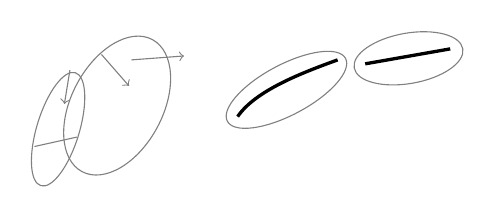
\begin{tikzpicture}[x=1cm,y=1cm]
\draw[gray,rotate around={-17:(.5,.6)}] (.5,.6) ellipse (.27 and .75);
\draw[gray,rotate around={-28:(1.25,.9)}] (1.25,.9) ellipse (.58 and .95);
\draw[gray,->] (.65,1.35)--(.58,.92);
\draw[gray,->] (1.05,1.55)--(1.40,1.15);
\draw[gray,->] (1.43,1.48)--(2.1,1.53);
\draw[gray] (.2,.38)--(.74,.5);
\draw[gray,rotate around={28:(3.4,1.1)}] (3.4,1.1) ellipse (.85 and .32);
\draw[very thick] (2.78,.76) .. controls (3.0,1.08) and (3.55,1.30) .. (4.05,1.48);
\draw[gray,rotate around={10:(4.95,1.5)}] (4.95,1.5) ellipse (.70 and .32);
\draw[very thick] (4.4,1.43)--(5.48,1.62);
\end{tikzpicture}}

\diagram{\begin{tikzcd}
F^0\arrow[r,shift left=.5ex]\arrow[r,shift right=.5ex]&
F^1\arrow[r,shift left=1ex]\arrow[r]\arrow[r,shift right=1ex]&F^2
\end{tikzcd}}
foncteurs $(\mathrm{Ens})\to(\mathrm{Ens})$

Objet simplicial de $\underline{\operatorname{Hom}}(\mathrm{Ens},\mathrm{Ens})$

Permet en principe de définir des $\pi_0,\pi_1$

$\pi_0(F)$, $F\in\underline{\operatorname{Hom}}(\mathrm{Ens},\mathrm{Ens})$, $F$
\[
F(I)\underset{?}{\simeq}C(K,I)
\]
$K$ espace top \uline{tot. discontinu}
[deux pts sont séparés par un ens : à la fois ouvert et fermé]

\uline{Cond néc} a) $F$ \unsure{permute|commute} aux
\deleted{produits} $\varprojlim$ finies

i.e. $F$ \uline{exact à gauche}
[donc $F$ transforme mon. en mon.]

b) \[
F(\bigcap I_\alpha)=\bigcap_\alpha F(I_\alpha)
\]
pour $(I_\alpha)$ famille filtrante de sous-ens. de $I$

Ces conditions équivalent à : \uline{$F$ strictement proreprésentable}
par un système projectif strict $(\pi_{0i})_i$ \deleted{\unsure{de}} d'ensembles.

Il faut de plus

c) \[
\deleted{\unsure{\pi_0F}}\quad
\varprojlim\pi_{0i}\longrightarrow\pi_{0i}
\quad\text{est \uline{surjectif} pour }\forall\,i.
\]

Ces conditions sont \uline{néc} et suffisantes, et on pourra prendre
$K=\varprojlim\pi_{0i}$, avec la topologie limite inverse des top. discrètes.

\uline{NB} Si $F$ est donné dans la forme $C(L,I)$, $L$ esp. top, homo
\[
\pi_0(L)\longrightarrow K.
\]
Si $L$ est \inserted{(quasi)} compact, cet homo est un
\unsure{isomorphisme|homéomorphisme}; \uline{en général}, ce n'est ni injectif, ni surjectif,

\margin{?\\Bourb. Topologie II\\p. 232, prop 6}
\scanpage{184}
% archive foliation: 183
\deleted{
\figure{\begin{tikzpicture}[x=.64cm,y=.64cm,>=stealth, every node/.style={font=\small}]
\node at (5.8,15.2) {\diagram{\begin{tikzcd}[column sep=small]
\overline K_0&
\overline K_1\arrow[l,shift left=.4ex]\arrow[l,shift right=.4ex]&
\overline K_2\arrow[l,shift left=.8ex]\arrow[l]\arrow[l,shift right=.8ex]
\end{tikzcd}}};
\draw (3.8,14.85)--(3.55,14.4);
\node at (3.45,14.15) {\unsure{fini}};
\draw (5.4,14.5)--(6.0,13.85);
\draw (7.35,14.45)--(6.8,13.95);
\node[align=center] at (6.4,13.45) {\unsure{qu. tot.}\\\unsure{disco}};
\node[font=\Large] at (9.7,13.8) {$A$};
\node[font=\Large] at (11.65,15.1) {$\mathbb Z$};
\node at (14.5,16.0) {$x$};
\node[font=\large] at (13.7,14.35) {$F$};
\node at (11.9,13.05) {$\unsure{k[[s,t]]}$};
\node at (11.85,12.25) {$\unsure{k\eta_1 ds}$};
\node[align=left,anchor=west] at (14.5,13.5)
{$\overline K_1-G$ \unsure{opère sur $\overline E$}\\[1ex]
de façon que $\overline K_1$ \unsure{$\gamma$} \uline{\unsure{que|soit}}\\[1ex]
\uline{continu}};
\draw[very thick] (14.4,12.25)--(15.1,13.0);
\node at (8.2,12.65) {\deleted{$f(x,y)$}};
\node at (10.1,12.15) {$\wedge$};

\draw[->,very thick] (.9,11.35)--(1.65,11.3);
\draw[->,very thick] (1.7,11.3)--(2.2,11.3);
\draw[->,very thick] (2.2,11.3)--(2.85,11.7);
\draw[->,very thick] (2.85,11.7)--(3.38,12.25);
\draw[->,very thick] (3.38,12.25)--(4.03,12.8);
\draw[->,very thick] (4.08,12.87)--(4.58,13.5);
\draw[->,very thick] (4.08,12.87)--(4.9,13.0);
\draw[->,very thick] (2.92,11.7)--(3.55,11.7);
\draw[->,very thick] (3.65,11.75)--(4.18,12.2);
\draw[->] (4.18,12.2)--(4.65,12.7);
\draw[->,very thick] (4.18,12.2)--(4.85,12.2);
\draw[->,very thick] (3.7,11.65)--(4.45,11.65);
\draw[->] (4.45,11.65)--(5.2,12.0);
\draw[->,very thick] (4.45,11.65)--(5.3,11.5);
\draw[->,very thick] (2.2,11.3)--(2.75,10.95);
\draw[->,very thick] (2.95,10.9)--(3.6,10.9);
\draw[->,very thick] (3.7,10.9)--(4.2,10.9);
\draw[->,very thick] (4.3,10.9)--(4.95,10.9);
\draw[->,very thick] (4.3,10.82)--(5.02,10.2);
\foreach \x/\y in {.9/11.35,2.2/11.3,2.85/11.7,3.38/12.25,4.03/12.8,3.55/11.7,4.18/12.2,2.75/10.95}
{\fill (\x,\y) circle (.05);}

\node at (9.05,11.05)
{$g(p(\unsure{t_1|u_1}))f(\unsure{t_1|u_1})g(q(\unsure{t_1|u_1}))^{-1}$};
\node[font=\large] at (9.15,9.95) {$\Pi_1^{\mathrm{eff}}(S,a)$};
\draw (7.35,9.55) .. controls (7.2,9.05) and (6.75,8.98) .. (6.55,9.0);
\draw (6.55,9.0) circle (.035);
\node[font=\large] at (4.85,9.15) {$\overline E$};
\draw (4.9,8.8)--(4.95,7.95);
\fill (4.95,7.8) circle (.02);
\draw[->,very thick] (.8,5.95)--(2.4,8.2);
\draw[->,very thick] (2.36,8.12)--(.78,5.9);
\draw[->] (.8,5.82)--(2.55,6.95);
\draw[->,very thick] (2.75,7.08) .. controls (3.12,7.62) and (2.8,8.1) .. (2.55,8.2);
\fill (2.4,8.3) circle (.03);
\fill (2.7,7.1) circle (.03);
\node at (2.85,5.55) {\deleted{$f(x,y)$}};
\node[font=\large] at (2.6,4.45) {$f(u)$};
\node[font=\Large] at (3.7,3.45) {$K_1$};
\node[font=\large] at (5.9,3.85) {$K_1$};
\fill (5.55,7.05) circle (.05);
\node[below] at (5.55,7.05) {$x$};
\fill (6.7,7.6) circle (.05);
\node[below] at (6.7,7.6) {$a$};
\draw[->,thick] (5.55,7.05)--(6.7,7.6);
\draw[->] (6.7,7.75) .. controls (7.85,9.2) and (6.4,9.0) .. (6.7,7.75);

\draw[->] (8.5,6.95)--(10.4,8.2);
\fill (10.55,8.35) circle (.02);
\draw[->] (10.6,8.5)--(11.25,10.2);
\fill (11.4,10.45) circle (.02);
\node at (11.8,10.6) {$b$};
\draw[->] (11.75,7.95)--(12.75,8.25);
\draw (13.0,8.3)--(13.55,8.65);
\draw[->] (13.75,8.8)--(14.15,9.5);
\fill (14.2,9.55) circle (.035);
\draw (14.2,9.95)--(14.5,10.45);
\draw (14.5,10.45) circle (.03);
\draw[->] (14.8,10.6)--(15.7,10.6);
\draw[->] (16.0,10.65)--(16.6,10.5);
\draw[->] (14.4,9.65)--(16.65,10.3);
\draw[->] (9.4,6.25) .. controls (11.2,7.1) and (9.35,8.4) .. (9.4,6.55);
\draw (9.4,6.25)--(10.1,6.6);
\node[font=\large] at (11.8,7.15) {$S\leftarrow S'$};
\node at (18.25,11.0) {$S$ connexe};
\node[draw,very thick,rectangle,font=\large] at (18.6,10.2)
{$\pi_1^{\mathrm{eff}}(S,a)$};
\node[font=\Large] at (17.4,8.8) {$S$};
\fill (17.45,9.5) circle (.025);

\fill (4.5,4.55) circle (.06);
\draw[->,very thick] (4.5,4.55)--(5.8,4.95);
\fill (5.95,4.95) circle (.045);
\node at (5.2,5.4) {$u_1$};
\draw[->,very thick] (5.95,4.95)--(6.85,5.55);
\draw[->,very thick] (7.0,5.6)--(7.55,6.6);
\draw[->,very thick] (7.0,5.5)--(8.0,5.5);
\node at (7.8,6.1) {$\unsure{b}$};
\draw[->,thick] (8.3,3.95)--(9.35,4.4);
\draw[->,thick] (9.45,4.45)--(9.95,5.0);
\draw[->,thick] (10.02,5.0)--(10.98,4.95);
\draw[->,very thick] (11.12,4.96)--(11.8,4.98);
\draw[->,very thick] (11.8,5.05)--(11.8,6.12);
\node[below] at (11.85,4.95) {$a$};

\draw[->,thick] (7.0,2.45) .. controls (5.95,4.0) and (8.1,5.0) .. (7.0,2.45);
\draw[->,thick] (7.25,2.42) .. controls (6.8,4.0) and (8.9,4.9) .. (7.25,2.42);
\draw[->,thick] (7.58,2.25) .. controls (7.4,3.7) and (9.4,4.7) .. (7.58,2.25);
\node at (7.8,1.25) {$\unsure{B}\leftarrow A$};
\fill (3.9,1.8) circle (.05);
\draw[->] (3.9,1.8)--(4.5,2.2)--(5.1,1.8)--(5.7,2.6);

\fill (10.2,2.65) circle (.05);
\node[below] at (10.2,2.65) {$a_0$};
\draw[->,thick] (10.55,2.65)--(13.45,2.7);
\draw[->,thick] (13.5,2.76)--(13.5,4.0);
\draw[->] (13.4,3.95)--(13.4,2.8);
\draw[->] (10.55,2.8)--(13.3,4.0);
\draw (13.47,2.7) .. controls (13.7,2.8) and (13.55,3.0) .. (13.5,3.2);

\fill (15.65,5.95) circle (.05);
\node[below] at (15.65,5.95) {$a$};
\draw[->,thick] (15.65,6.1)--(15.05,8.05);
\node at (14.95,8.45) {$\unsure{c|E}$};
\draw[->] (15.9,6.05) .. controls (16.4,6.7) and (16.4,7.0) .. (16.6,7.4);
\node at (16.7,7.65) {$b$};
\draw[->,thick] (16.35,7.8)--(15.45,8.2);
\node at (16.0,8.35) {$d_2$};
\node at (14.85,6.75) {$d_1$};
\node at (16.6,6.75) {$d_0$};
\draw[->] (15.7,8.08)--(15.3,7.1);
\draw[->] (15.95,7.9)--(15.6,6.95);
\draw[->] (16.15,7.78)--(15.85,7.02);
\node at (12.48,4.45) {$x$};
\draw[->,thick] (14.7,7.9)--(12.65,4.75);
\draw[->] (12.5,4.5)--(14.6,7.9);
\draw[->,thick] (16.15,7.3)--(12.88,4.65);
\draw[->] (12.7,4.5)--(16.6,7.4);
\draw[->,thick] (12.72,4.52)--(15.35,5.95);
\draw[->] (15.1,5.75)--(12.8,4.4);

\draw[->,very thick] (18.3,5.65)--(19.18,6.05);
\draw[->,thick] (19.1,6.25)--(18.15,5.88);
\draw[->,very thick] (19.18,6.05)--(19.45,7.0);
\draw[->,thick] (19.2,7.03)--(18.98,6.3);
\draw[->,very thick] (19.45,7.0)--(20.3,7.4);
\draw[->,thick] (20.25,7.6)--(19.35,7.2);
\draw[->,very thick] (20.3,7.4)--(20.5,8.4);
\draw[->,thick] (20.3,8.35)--(20.1,7.5);
\node at (20.75,8.5) {$a$};
\draw[->] (18.2,5.45) .. controls (19.5,5.65) and (19.9,6.8) .. (19.7,7.1);
\draw (20.5,7.95) circle (.02);

\node at (14.55,3.3) {$x$};
\draw[->,thick] (17.75,4.55)--(15.0,3.4);
\draw[->] (15.05,3.5)--(17.8,5.75);
\draw[->,thick] (18.05,4.95)--(17.75,5.85);
\draw (14.65,3.2)--(17.7,4.4);
\node at (17.15,2.75) {$x$};
\draw[->,thick] (17.48,2.9)--(18.1,3.22);
\draw[->] (18.0,3.4)--(17.42,3.08);
\node[below] at (17.85,2.95) {$u_n$};
\draw[->,thick] (18.32,3.42)--(19.12,3.78);
\draw[->] (19.02,3.96)--(18.28,3.6);
\node[below] at (18.8,3.5) {$u_{n-1}$};
\draw[->,thick] (19.48,4.0)--(20.2,4.37);
\draw[->] (20.06,4.57)--(19.43,4.2);
\node[below] at (19.96,4.02) {$u_1$};
\node at (20.35,4.32) {$a$};
\draw[->,thick] (13.0,1.5)--(15.7,2.62);
\draw[->,thick] (15.58,2.8)--(12.9,1.66);

\draw[thin] (2.2,14.9)--(20.4,3.85);
\draw[thin] (1.8,10.3) .. controls (4.0,7.9) and (10.0,4.2) .. (15.4,1.05);
\draw[thin] (13.0,15.5)--(19.7,10.55);
\end{tikzpicture}}
}
\scanpage{185}
% archive foliation: 184
mais il est naturel de mettre sur $\pi_0(L)$ la topologie image inverse de
$K$ topologie \inserted{\unsure{de|des} $\pi_0(L)$} [des partitions ouvertes de $L$].
$F$ est dit \uline{connexe} si $F\simeq\mathrm{id}_{\mathrm{Ens}}$,
i.e. $F$ est $T$-représentable par l'espace ponctuel
[i.e. par un espace connexe].

Considérons deux \deleted{foncteurs} flèches
\diagram{$F^*:$\quad\begin{tikzcd}
F^0\arrow[r,shift left=.5ex]\arrow[r,shift right=.5ex]&F^1
\end{tikzcd}
$\qquad (F^0,F^1\in\underline{\operatorname{Hom}}(\mathrm{Ens},\mathrm{Ens}))$}
et le \uline{foncteur noyau}
\[
\Pi^0(F^*)=F=\operatorname{Ker}(F^0\rightrightarrows F^1)
\]
Si $F^0,F^1$ sont \deleted{\unsure{strictement pro}}\inserted{$T$-}représentables,
alors les deux flèches proviennent de flèches
\diagram{\begin{tikzcd}
K_0&K_1\arrow[l,shift left=.5ex]\arrow[l,shift right=.5ex]
\end{tikzcd}}
et $F$ sera également $T$-représentable
[N.B. Toute $\varprojlim$ de foncteurs $T$-représentables est $T$-repr,
en prenant une limite inductive sur les espaces dont ils proviennent,
\deleted{$\unsure{\xi}$} et le $\pi_0$ associé].
Un couple de $F^{\unsure{\alpha|*}}$ comme dessus est dit
\uline{connexe} si son noyau est connexe.

Considérons un ``foncteur \unsure{cosimplicial}'',
\inserted{\unsure{objet simplicial de}}
de $\underline{\operatorname{Hom}}(\mathrm{Ens},\mathrm{Ens})$
\diagram{\begin{tikzcd}
F^0\arrow[r,shift left=.5ex]\arrow[r,shift right=.5ex]&
F^1\arrow[r,shift left=1ex]\arrow[r]\arrow[r,shift right=1ex]&F^2
\end{tikzcd}}
On lui associe foncteurs $\Pi^0(F^*;E)$,
\deleted{\unsure{G}} et $\Pi^1(F^*;G)$,
où $E$ ens variable, $G$ groupe variable.
Si $F^*$ est \uline{coponctué} i.e. muni de
$F^*\to\mathrm{id}_{\mathrm{Ens}}^*$, on définit des $=$
$\Pi^0(F^*,\unsure{\zeta|\xi};E)$ et
$\Pi^1(F^*,\unsure{\zeta|\xi};G)$, $\unsure{\zeta|\xi}$
\scanpage{186}
% archive foliation: 185
désignant la ponctuation. Plus généralement, si on a un autre foncteur
\inserted{co}simplicial
\diagram{\begin{tikzcd}
f^0\arrow[r,shift left=.5ex]\arrow[r,shift right=.5ex]&
f^1\arrow[r,shift left=1ex]\arrow[r]\arrow[r,shift right=1ex]&f^2
\end{tikzcd}}
\deleted{\unsure{on va de}} et un hom \inserted{co}simplicial $\unsure{\zeta|\xi}$
\diagram{$\unsure{\zeta|\xi}:$\quad
\begin{tikzcd}[row sep=large]
F^0\arrow[r,shift left=.5ex]\arrow[r,shift right=.5ex]\arrow[d,"\unsure{\zeta^0|\xi^0}"']&
F^1\arrow[r,shift left=1ex]\arrow[r]\arrow[r,shift right=1ex]\arrow[d,"\unsure{\zeta^1|\xi^1}"']&
F^2\arrow[d,"\unsure{\zeta^2|\xi^2}"']\\
f^0\arrow[r,shift left=.5ex]\arrow[r,shift right=.5ex]&
f^1\arrow[r,shift left=1ex]\arrow[r]\arrow[r,shift right=1ex]&f^2
\end{tikzcd}}
on définit $\Pi^0(F^*,\unsure{\zeta|\xi};E)$ et
$\Pi^1(F^*,\unsure{\zeta|\xi};E)$.

Si $F^0,F^1,F^2$ sont $T$-représentables, et dans le cas où on se donne
des $\unsure{\zeta|\xi}:F^*\to f^*$, si $f^*$ est $T$-représentable,
on ramène ceci à la donnée d'un \deleted{objet} \uline{espace simplicial}
\diagram{\begin{tikzcd}
K_0&K_1\arrow[l,shift left=.5ex]\arrow[l,shift right=.5ex]&
K_2\arrow[l,shift left=1ex]\arrow[l]\arrow[l,shift right=1ex]
\end{tikzcd}}
resp d'un \uline{espace simplicial} \uuline{ponctué} (par contraction)
\diagram{\begin{tikzcd}
\overline K_0&\overline K_1\arrow[l,shift left=.5ex]\arrow[l,shift right=.5ex]&
\overline K_2\arrow[l,shift left=1ex]\arrow[l]\arrow[l,shift right=1ex]
\end{tikzcd}}
par un procédé standard \unsure{----}.

Il y a lieu de généraliser ces constructions au cas où
\unsure{sur des} $K_i$, resp. des $\overline K_i$, on a des catégories
galoisiennes attachées à chaque pt,
\deleted{\unsure{(connexes, les $F^i$}}
pour décrire des relations de descente à la
\uline{Van Kampen} \unsure{-----}
\scanpage{187}
% archive foliation: 186
\uline{Proposition}\quad Soit $f:X-Y$ un morphisme, avec
\[
\left|
\begin{array}{ll}
1)&\deleted{f\text{ loc de présentation finie et loc quasi-fini}}\\[-.3ex]
 &\inserted{Y\text{ loc. noeth et univ. japonais}}\\
2)&\deleted{\unsure{Y}}\ X\quad\deleted{\text{irréductible}}\ 
\text{n'a qu'un nb fini de comp irred.}\\
3)&f\text{ loc. }\inserted{\uline{\text{de type fini}}}
\text{quasi-fini}\quad\deleted{\text{et, et}}\quad f\ \uline{\text{séparé}}
\end{array}
\right.
\]
\[
\left|\quad\text{Dans ces conditions, }f\text{ est \uline{de type fini}.}\right.
\]

On peut supposer $Y$ affine donc noeth, \unsure{\&}
$X$ intègre \deleted{et $f$ dominant}
\inserted{(car il suffit de voir que $f$ est quasi. cpt)}.
Soit $U$ un ouvert \inserted{affine} non vide de $X$, il est
quasi-fini séparé sur $Y$, donc par le main theorem il est
$Y$-isomorphe à un ouvert $\unsure{U|U'}$ d'un $Y$-\deleted{\unsure{entier alg}}
préschéma \uline{fini} $X'$, qu'on peut supposer intègre.

\margin{\diagram{\begin{tikzcd}[column sep=large,row sep=large]
&X''\arrow[dl,"\text{fini}"']\arrow[d]\\
X\arrow[d]&X'\arrow[dl,"\substack{\text{fini}\\\unsure{\text{surj}}}"]\\
Y&
\end{tikzcd}}}

Soit $X''$ le sous-préschéma fermé intègre de $X\times_YX'$
\deleted{\unsure{par prolongement}}
\inserted{adhérence de}
la ``diagonale'' de $U\times_YU'$, donc $X''$ s'envoie dans $X$ et $X'$.
Mais $X''-X$ est fini, et étant dominant, est \uline{surjectif}.
Il suffit donc de voir que $X''$ est de t.f. sur $Y$, ou même sur $X'$.
Or $X''-X'$ est un morphisme birationnel, avec $X''$ et $X'$ intègres.
Donc \deleted{\unsure{il}} y a un $X'$-morphisme
\deleted{\uline{surjectif}} $\widetilde X'-X''$, où $\unsure{X'|\widetilde X'}$
est le normalisé. Or $\unsure{X'|\widetilde X'}$ est fini sur $Y$,
on \unsure{gagne} \unsure{.....}
